

\chapter{\textit{Like}: Frequency and phonetic realisations}
\label{ch:prod}
\date{}
%\maketitle

\section{Methodology of interviews}\label{interview:method}

In a standard sociolinguistic interview, an interviewer asks questions designed to elicit the ``vernacular'', which is essentially the range of speech styles used in informal situations when there is no interviewer present.\footnote{`Vernacular' has been defined a number of different ways, including Labov's original definition of the term as ``the style in which the minimum attention is given to the monitoring of speech'' (Labov 1972: 208).  \citeasnoun{milroy1992} defines the term as ``real language in use''.  I have put the term in quotation marks because I view speech styles as points along multidimensional continua and am dubious of the ability to identify and label some portion of these continua as the vernacular.}  Questions, such as whether the interviewee has ever had a near-death experience, are used to shift the focus from \textit{how} the narrative is said to the content of the narrative itself.  Often followed by read passages and/or wordlists, the traditional Labovian style interview is a popular method to elicit speech, as it provides a means of lessening the effects of the Observer's Paradox.  As speakers become more involved in the interaction, they become less focused on the fact that they are being recorded \cite{labov1972sociolingpatterns}.  I adopted an alternative approach for my interviews at Selwyn Girls' High for the following reasons:\footnote{I use the word \textit{interview} to refer to a conversation that was recorded, even when it was not in a format traditionally used for interviews.  This term is used to distinguish these conversations from interactions that were not recorded but were written in my fieldnotes.} 



\begin{enumerate}

\item[(1)] Previous work has shown that greater familiarity with an outsider decreases the amount a speaker will accommodate, thereby reducing the effect of the Observer's Paradox \cite{cukoravilabailey}. I did not begin recording until I had spent two months at the school, so I was already familiar with the girls at the time of the interviews.

\item[(2)]  The Observer's Paradox was lessened even further through conducting multiple recorded interviews with many of the individual girls.  They became more comfortable with the recording equipment after multiple encounters.  

\item[(3)] Speakers are less likely to accommodate to the speech of a researcher if family members or peers are present \cite[115]{labov1972principles}.  Most of the interviews I conducted were with at least two girls.

\item[(4)]  As a way of maintaining naturalness, I gathered recordings of conversations between different girls rather than between myself and them.  In addition to preserving naturalness, I used this technique because I was interested in documenting what they talked about with each other as opposed to what they talked about with me. 
\end{enumerate}

\noindent I conducted two different types of interviews depending on the situation.  One involved multiple interviewees and spontaneous conversation between them and the other was an unstructured one-on-one interview.  I will step through these in more detail shortly.  In both types of interviews, girls asked what I was interested in and whether I had any findings thus far.  I used these questions as an opportunity to ask about the social make-up of the school and how they viewed their own identity.  

I most frequently used the first type of interview, which involved approaching girls who were already in conversation and asking if I could record them.  Sometimes the place of conversation was too noisy for a quality recording and I suggested moving the conversation to a quieter room.  After shifting rooms, the girls would continue the conversation where they left off, though they usually included me in the conversation for at least a part of the interview.   

This technique had drawbacks, as there were girls who I was interested in interviewing but who I had not seen interacting with a group small enough to be suitable for recording.  With these girls, I conducted one-on-one interviews that involved questions and answers by both of us.  As a result, the role I played in the conversations varied across the different types of interviews.  While there were bound to be linguistic differences as a result of these different interview techniques, it did not significantly affect the sociophonetic analysis presented in Section \ref{sec:phoneticlike}; individual girls who took part in the two interview types produced similar variants of \textit{like} across both.\footnote{The type of interview was tested statistically as a predictor for realisation in model 2, which is presented in Section \ref{sec:phoneticlike}. It was not found to influence production on its own (p = 0.93), providing statistical evidence that the different token types were evenly distributed across the different interview types, nor was it found to be involved in an interaction with /k/ realisation (p = 0.33), providing evidence that the interaction between /k/ realisation and social group is not an artefact of interview type.}  
%Variation of other phonetic variables depending on the different interview types is an intended area of investigation for the future.

I had time on my side, so I invited all girls to ask me questions in addition to any I might ask.  I did not want the interview to have an unbalanced distribution of power based on the interviewer-interviewee relationship and I chose instead to emphasise solidarity by highlighting our equality in the interactions.  As a result, there are portions of some interviews where I talked extensively.  Of course, this loose interview style would not suit researchers interested in eliciting the maximum amount of speech in the minimum amount of time.  However, spending four days a week among the girls for an entire school year meant that I had enough contact time to use the most naturalistic context possible.

Recordings were made in various places on the school grounds (a classroom, the common room, or outside if it was sunny) using a table microphone (AKG:C543BL) and a Marantz solid state recorder (PMD670), which records directly onto a CompactFlash digital memory card. 


\section{Variation in use of \textit{like}}\label{prod-like}


A select number of recorded interviews with the girls were transcribed using the tool Transcriber (Barras et al. 2000), resulting in a transcribed corpus of over 15 hours of speech from 59 different girls.\footnote{Due to the sensitive nature of some interviews and the criteria set out by the Human Ethics Committee at the University of Canterbury, all recordings were transcribed by me.}  
\nocite{Transcriber-SpeechComm2000}

The analysis presented in this chapter focuses on the speech of 28 girls, 14 of whom were CR girls.  All girls whose speech was analysed took part in the perception experiments presented in Chapter \ref{ch:perc}.\footnote{I focused on transcribing interviews with girls who had participated in the experiments so that I could compare patterns of phonetic variables in their production to patterns of their responses during perception.}  Of the 42 girls who took part in the perception experiment, the 14 CR and 14 NCR girls who had the most speech recorded in the interviews were analysed. This was done in order to identify a large enough number of tokens for each speaker on which to conduct the statistical analysis.   The individual girls whose speech was analysed are shown in Appendix \ref{app:socialgroups}.   Table \ref{tab:groupsprod} displays the number of girls from each of the individual subgroups whose speech was analysed.

\begin{table}[htbp]
\caption{The number of speakers in each subgroup that were analysed.}	
	\label{tab:groupsprod}
	 \begin{center}
		\begin{tabular}{lrlr}
		\lsptoprule
		\sc cr Group & \sc speakers & \sc ncr group & \sc speakers \\
  \midrule
The PCs & 3      &Pasifika Group & 1  \\
Sporty Girls & 3  &The Goths & 5 \\
Trendy Altern. & 3  &The Geeks & 3  \\
Rochelle's Group & 1   &Real Teenagers & 2 \\
Relaxed Group & 3      &Christians & 2 \\
The BBs & 1        &Sonia's Group & 1  \\\midrule
\sc total & 14  & & 14  \\

\lspbottomrule
		\end{tabular}
	
	\end{center}
\end{table} 


\noindent A great deal of variation can be found in the girls' speech.  In the interest of investigating subtle differences in pronunciation across social groups as well as across different meanings of a single word, this chapter focuses on variation within the word \textit{like}.  The type of phonetic analysis that I conducted is time-consuming, particularly since I coded for a wide range of phonetic information.  Given time constraints, it would not have been possible to examine these phonetic variables across a range of words without losing the theoretical insights gained from examining phonetic variation of lemmas that share an identical lexical form.  These insights are discussed in Section \ref{sec:proddisc}.

The word \textit{like} was chosen for analysis because several of the different meanings of \textit{like} were highly frequent in all of the girls' speech.  This made it possible to conduct a within-speaker analysis of the realisations produced in spontaneous speech.  Additionally, I hypothesised that socially-conditioned phonetic variation could arise depending on the nature of the different functions of \textit{like}: some of the functions are traditionally grammatical while others are discursive and are themselves layered with social meaning. Given that they were highly salient at the school and were ideologically linked with youth culture (and with certain individual girls at the school, in particular), \textit{like} seemed like a promising lexeme to focus on.  I was particularly interested to see whether different individuals and groups of speakers produced different realisations that varied - not only according to their social group - but also depending on the token's grammatical function.  For example, might there be a difference between groups in the pronunciation of a discourse-pragmatic function of \textit{like} (discussed below) that is not observed for the more grammatical functions (e.g., the lexical verb)?  

Furthermore, I am interested in the relationship between the phonetic realisation of a word and the word's probability of occurrence. I hypothesized that the likelihood that a speaker will producs a certain word might influence that speaker's pronunciation of the word.  Focusing on the word \textit{like} allowed me to test this hypothesis (1) because I could control for word-internal phonological factors and (2) all of the girls produced tokens of \textit{like} though they did so to varying degrees.

Although this chapter focuses on phonetic variation in the word \textit{like}, there was a great deal of other phonetic variation in the recordings.  This variation has not yet been analysed systematically.  However, I intend to examine it in more depth in the future.  

For the analysis of \textit{like}, I used the different grammatical and discursive functions of \textit{like} as outlined by \citeasnoun{darcy2007}.  Among its grammatical functions, \textit{like} may be a lexical verb (\ref{item:lexV}) or an adverb (\ref{item:adv}).  These were the most frequent of the grammatical functions of \textit{like} found in the SGH data.  Other grammatical functions of \textit{like} are the noun (\ref{item:noun}), the conjunction (\ref{item:conj}), and the suffix (\ref{item:suffix}).  The examples listed here are from \citeasnoun{darcy2007}.


\sents{

\item  Lexical Verb:	I don't really LIKE her that much.\label{item:lexV} 

\item	Adverb:	It looks LIKE a snail; it just is a snail.\label{item:adv}

\item	Noun:	He grew up with the LIKES... of all great fighters.\label{item:noun}

\item  Conjunction: It felt LIKE everything had dropped away.\label{item:conj}

\item	Suffix:	I went (mumbling) or something like stroke-LIKE.\label{item:suffix}
\label{gramlikes}
}

\noindent The word \textit{like} also has discursive functions.  It can serve as a discourse marker (\ref{item:dm}), a discourse particle (\ref{item:dp}), an approximative adverb (\ref{item:approxadv}), or a quotative (\ref{item:quote}).  All of the discursive functions occur frequently in the speech of girls at SGH.  The examples presented here are taken from interviews with the girls.

\sents{

\item  Discourse marker:	LIKE it real cracks me up. (Emma, The PCs, 26-10)\label{item:dm}

\item  Discourse particle:	Lily was LIKE checking out my bro\-ther. (Ka\-na\-ni, The Spor\-ty Girls, 24-07)\label{item:dp}

\item  Approximative adverb: I did that in LIKE two days. (Theresa, The Christians, 20-09)\label{item:approxadv}

\item Quotative:	and Mum's LIKE ``turn that stupid thing off.'' (Marama, The Pasifika Group, 02-11)\label{item:quote}
\label{disclikes}
}

\noindent The lexical verb, adverb, quotative, and discourse particle were chosen for analysis because they were highly frequent, meaning that there were sufficient data for statistical analysis of their phonetic realisations.  While the discourse marker is also highly frequent, it occurs at the beginning and end of phrases whereas the analysed functions of \textit{like} most often occur phrase-medially.\footnote{Included in the analysis were tokens of quotative \textit{like} where the remainder of the sentence was a gesture.}

Quotative \textit{like} can be used in a variety of different situations.  For example, it can be used to report speech, thoughts, and gestures \cite{romainelange1991}.  The analysis presented here combines all of the different pragmatic functions of quotative \textit{like} into a single category though it is possible that they could have different distributions or phonetic realisations.\footnote{An analysis of the different pragmatic functions of quotative \textit{like} revealed no function-based variation in these data, but this may be due to the relatively small number of tokens of each function.}



\subsection{Use of quotative \textit{like} at SGH}\label{section:uselike}



The frequency of use of the different types of \textit{like} varied depending on the individual.  Based only on girls whose speech was analysed, two calculations were made with the aim of approximating a speaker's likelihood of using quotative \textit{like}.  I decided to use two calculations because (a) frequency of use has been measured previously on the basis of both calculations and (b) I wanted to provide the most complete picture of the distribution of quotative \textit{like} among the girls.

The first measure of frequency of use of the quotative was the average number of times a token of quotative \textit{like} was produced for every hundred words produced by a speaker.\footnote{Word counts were generated automatically using ONZE Miner.  Words with hyphens (e.g., \textit{ex-boyfriend}) were counted as a single word.}  A raw count of the quotative would not be representative of frequency of use due to differences in interview length across different girls.  Though frequency of use is usually normalised per one thousand words, a smaller corpus necessitates normalising per one hundred \cite[264]{biberetal1998}.  The measure is shown, by increasing use of quotative \textit{like}, in Table \ref{tab:percentquote}.  Token frequency measures are usually based on corpora, such as CELEX, that contain millions of words, but this is not realistic for examining speaker-specific frequencies.  In the current study, the already relatively small word count of the corpus was made even smaller through examining intraspeaker frequency of use.  Therefore, the values presented in Table \ref{tab:percentquote} should be viewed with some caution.
  
  
  

  \begin{table}[htbp]
\caption{Values based on the first measure of frequency of use of quotative \textit{like}: The number of tokens of quotative \textit{like} per hundred words produced, ordered by increasing usage of quotative \textit{like}.  Also shown is the number of all other quotatives by hundred words produced.}
  \label{tab:percentquote}
	 \begin{center}
		\begin{tabular}{lld{0}d{4}d{4}}
		\lsptoprule
\sc group & \sc cr/ncr &  \multicolumn{1}{c}{\sc total words} & \multicolumn{1}{c}{\sc quotative \textit{like}} & \multicolumn{1}{c}{\sc other quotatives} \\
		 \midrule

Patricia	& \sc cr &  4629	& 0.1080 & 0 \\
Santra	& \sc ncr & 6462	& 0.2786 & 0.2321 \\
Marissa	& \sc ncr & 1238	& 0.3231 & 0.1616 \\
Marama & \sc ncr & 	2783	& 0.3234 & 0.2515 \\
Mariah & \sc ncr & 	6126	& 0.3265 & 0.0490 \\
Juliet & \sc cr & 1032 &	0.3876 & 0.2907 \\
Christina	& \sc cr & 1440	& 0.4167 & 0.0694 \\
Tania	& \sc ncr & 3945 &	0.4309 &  0 \\
Katrina	& \sc cr & 1572 &	0.5089 & 0.0636 \\
Esther & \sc ncr &	4532	& 0.5296 &  0.0662 \\
Vanessa	& \sc ncr & 4728	& 0.5499 &  0.1904 \\
Justine	& \sc cr & 2022	& 0.5935 &  0 \\
Barbara	& \sc cr & 2867	& 0.6278 &  0.2442 \\
Bianca	& \sc ncr & 4197	& 0.6671 & 0.2144 \\
Clementine & \sc cr & 	3093	& 0.6790 &  0.1940 \\
Emma & \sc cr &	3916	& 0.7916 &  0.0255 \\
Jane	& \sc cr & 1236	& 0.8900 &  0.0809 \\
Theresa	& \sc ncr & 1279	& 1.0164 &  0.2346 \\
Sarah	& \sc ncr & 2150	& 1.1163 & 0.0465 \\
Rochelle & \sc cr &	1850	& 1.1351 & 0.1622 \\
Meredith	& \sc ncr & 6815	& 1.2032 & 0.1321 \\
Isabelle	& \sc ncr & 6776	& 1.5939 & 0.1476 \\
Betty	& \sc cr & 1040	& 1.6346 & 0.1923 \\
Tracy	& \sc cr & 1157	& 2.0743 & 0.1729 \\
Kanani & \sc cr	& 1769	& 2.0916 & 0.1696 \\
Rose & \sc cr &	3653	& 2.4090 & 0.1369 \\
Holly	& \sc ncr & 2878	& 3.1619 & 0.0695 \\
Joy & \sc ncr &	683	& 3.5139 & 0.1464 \\\midrule
 & &  \text{\sc total:~} 85868	& \text{\sc mean:~} 1.0494 & \text{\sc mean:~} 0.1337 \\

\lspbottomrule
		\end{tabular}
	
	\end{center}
\end{table} 

Also shown in Table \ref{tab:percentquote} is the number of all other quotatives (i.e. quotatives that were not \textit{like}) per hundred words produced.  When comparing the two normalised frequency measures, it is evident that while some speakers, such as Patricia, had low counts of quotative \textit{like} but produced few quotatives overall, other speakers, such as Santra, produced a large number of quotatives but used other quotatives nearly as much as they used quotative \textit{like}.  

The second measure was the percentage of all quotatives that were quotative \textit{like}, a calculation that follows the Principle of Accountability \cite{labov1972sociolingpatterns}.  Because not all speech acts (and therefore not all recorded interviews) necessitate the use of quotatives, this measure provides a means of comparing the use of quotative \textit{like} across speakers within the context of other quotatives they might use instead; it is a reflection of how likely a speaker was to use quotative \textit{like} rather than one of the alternatives available.  Therefore, it is a measure of token probability, which is related to but also distinct from token frequency.

Bybee's (2002) interpretation of the relationship between token frequency and phonetic reduction depends on overall token counts.  This means that in collecting counts of speaker-specific token frequency, a researcher would need to record all interactions in which a speaker is involved over an extended period of time.  Interpreting the measures of frequency presented here in terms of their reflection of speaker-specific token frequency is problematic because (1) some speakers, in general, may be less likely to use reported speech than others, (2) some speakers, in general, may talk more than other speakers, and (3) the recordings may not be equally distributed across speakers for different types of speech acts.  While the second measure can control for the latter of these concerns, it is less clear how to account for the first two.  The first measure, however, does not control for any of these concerns. Therefore, the measures presented here are not analogous to token frequency, but instead are informative of the relative frequency of a token.  The first is the frequency relative to the number of words produced in the interaction and reflects the probability that, regardless of the speech act, a token will be quotative \textit{like}.  The advantage of this measure is that not all girls may use the same amount of reported speech.  However, this measure is problematic in that it assumes that the ratio of total speech to reported speech is equivalent to what would be observed across all interactions with the speakers, which is unlikely given the small number of interviews analysed.  For this reason, this measure should be viewed with some caution.  For the second measure, the frequencies are relative to the frequency of alternative quotatives that could be used.  This reflects the probability that, if producing a quotative, the quotative will be \textit{like}.  This measure of probability assumes that the ratio of quotative \textit{like} to the other quotatives used by a speaker reflects the ratio used by that speaker in interactions that were not recorded.

\nocite{bybee2002-lvc}

\begin{table}[htbp]
\caption{Values based on the second measure of frequency of use of quotative \textit{like}: The percentage of all quotatives produced by a speaker that were quotative \textit{like}, ordered by increasing usage of \textit{like}.}
  \label{tab:percentlike}
	 \begin{center}
		\begin{tabular}{lld{0}d{2}}
		\lsptoprule
	
\multirow{2}{*}{\sc speaker} & \multirow{2}{*}{\sc cr/ncr} & \multicolumn{1}{p{2cm}}{\centering\sc total\newline quotatives} & \multicolumn{1}{p{2.5cm}}{\centering\sc \% quotative\newline \textit{like}}\\
  \midrule
Santra &	\sc ncr &	33	& 54.55 \\
Marama &	\sc ncr	& 16	& 56.25 \\
Juliet &	\sc cr	& 7	& 57.14 \\
Marissa	& \sc ncr	& 6	& 66.67 \\
Barbara	& \sc cr	& 25	& 72.00 \\
Vanessa	& \sc ncr	& 35	& 74.29 \\
Bianca	& \sc ncr	& 37	& 75.68 \\
Clementine	& \sc cr	& 27	& 77.78 \\
Theresa	& \sc ncr	& 16	& 81.25 \\
Christina	& \sc cr	& 7	& 85.71 \\
Mariah	& \sc ncr	& 23	& 86.96 \\
Rochelle	& \sc cr	& 24	& 87.50 \\
Esther	& \sc ncr	& 27	& 88.89 \\
Katrina	& \sc cr	& 9	& 88.89 \\
Betty	& \sc cr	& 19	& 89.47 \\
Meredith	& \sc ncr	& 91	& 90.11 \\
Isabelle	& \sc ncr	& 118	& 91.53 \\
Jane	& \sc cr	& 12	& 91.67 \\
Tracy	& \sc cr	& 26	& 92.31 \\
Kanani	& \sc cr	& 40	& 92.50 \\
Rose &	\sc cr	& 93	& 94.62 \\
Joy	& \sc ncr	& 25	& 96.00 \\
Sarah	& \sc ncr	& 25	& 96.00 \\
Emma &	\sc cr	& 32	& 96.88 \\
Holly	& \sc ncr	& 93	& 97.85 \\
Justine	& \sc cr	& 12	& 100 \\
Patricia	& \sc cr	& 5	& 100 \\
Tania	& \sc ncr	& 17	& 100 \\\midrule
& & \text{\sc total:~} 900	& \text{\sc average:~} 85.09 \\

\hline
		\end{tabular}
	
	\end{center}
\end{table} 

Table \ref{tab:percentlike} shows the percentage of all quotatives produced by a speaker that were quotative \textit{like}.\footnote{The null quotative (reported speech without the use of a quotative verb) is difficult to search for and was not included in the count.  Though the null quotative can account for as much as 20\% of quotatives in other dialects, such as Canadian English \cite{tagliamontehudson1999}, during transcription it was noted that though the null quotative was observed, it was infrequent in the speech of the SGH girls.  Furthermore, work in New Zealand has found low rates of the null quotative among females of a similar age to the girls in the current study \cite{buchstallerdarcy2009}.}  Quotative \textit{like} was the most common quotative for all of these speakers, accounting for the majority of quotative tokens for all 28 girls.  Nonetheless, there was some variation in its frequency of use.  It was least frequent in the speech of Santra (Goths), Marama (Pasifika Group), and Juliet (PCs) and it was most frequent in the speech of Justine (Trendy Alternatives), Patricia (Sporty Girls), and Tania (Goths).  This will be discussed further alongside discussion of the alternative quotatives sometimes used.


The two measures for the speaker-specific frequency of quotative \textit{like} are statistically correlated (Spearman's rho = 0.46; p$=$0.01).  This is expected given that both measures are based on the number of tokens of quotative \textit{like} for each speaker.  However, notice how for some speakers with a low number of overall quotatives (e.g., Patricia, Tania, and Justine) the two sets of values are very different in terms of how the girls are ranked in their respective frequencies of use. It is likely that this is a result of calculating the first measure over the relatively small amount of speech recorded for each speaker.  This emphasises the importance of analysing quantitative data in terms of the context in which it is relevant when working with a small corpus.  

In both measures, CR girls produced more tokens of quotative \textit{like} than NCR girls, as shown in the boxplots in Figure \ref{fig:ComparingQLikeMeasures}. However, the difference between CR and NCR girls was not significant for either measure (Wilcoxon, p = 0.25, p = 0.8).  

\begin{figure}
	\centering
		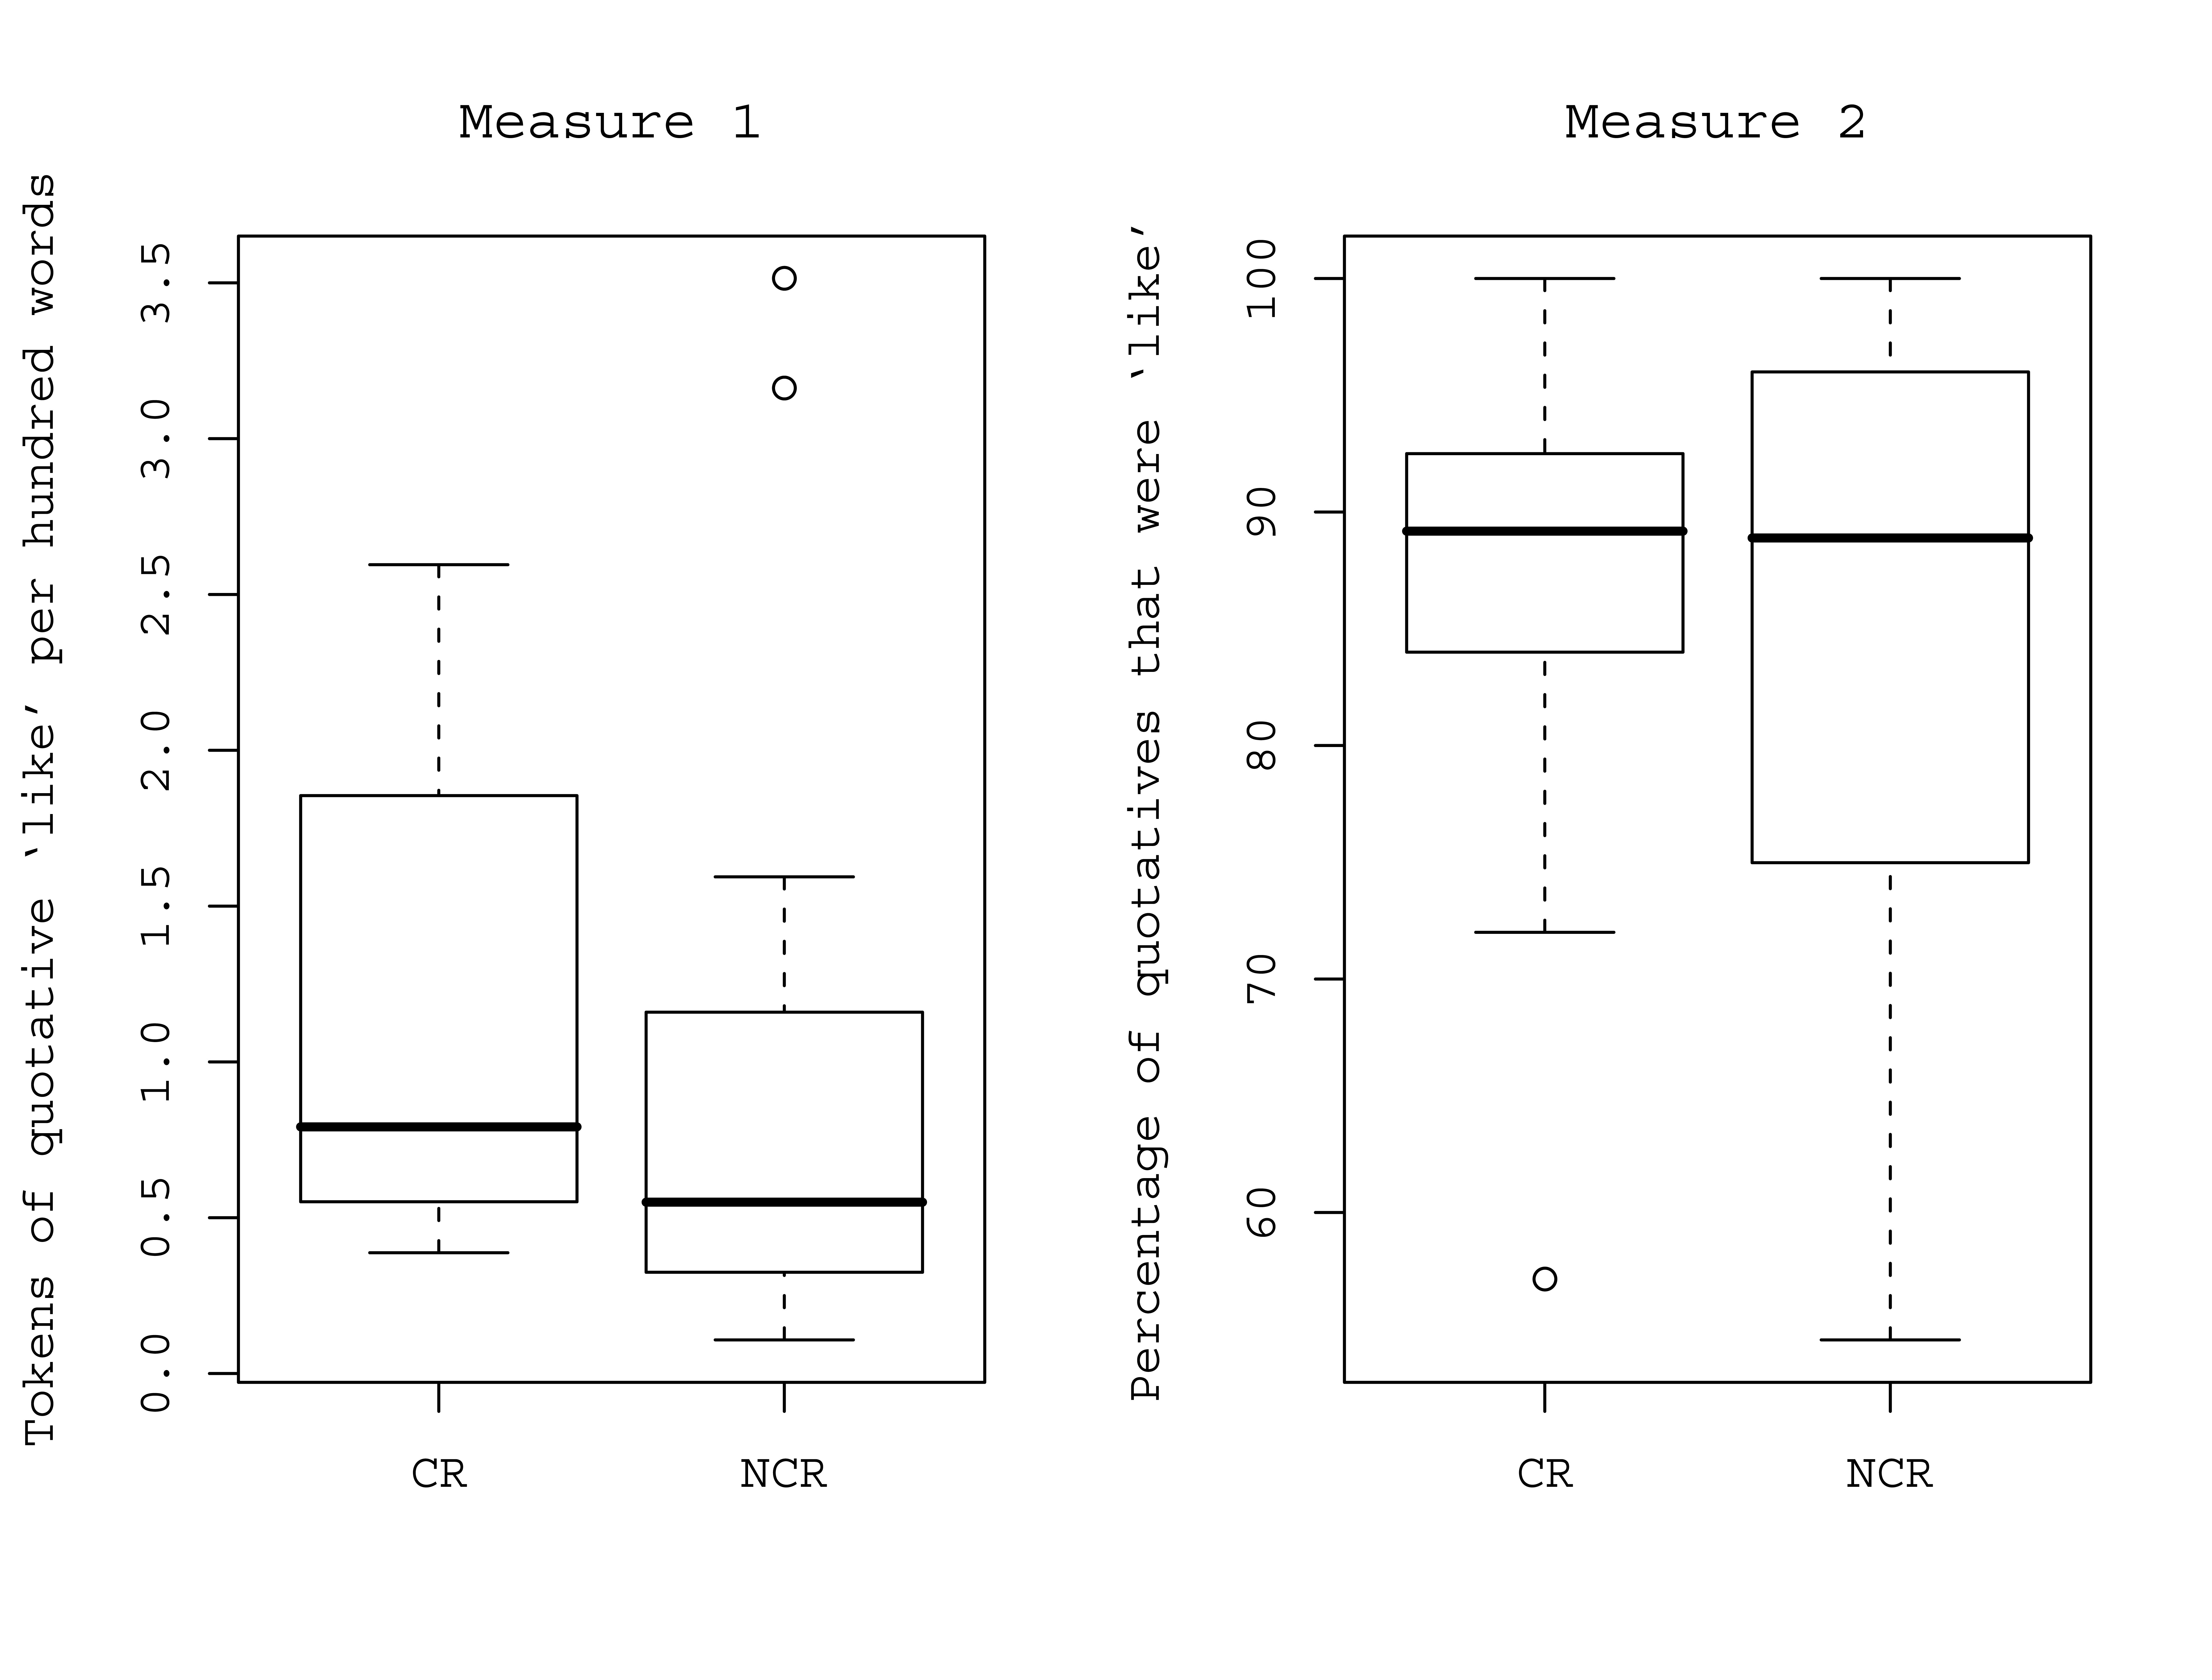
\includegraphics[width=5in]{images/ComparingQLikeMeasures.jpg}
	\caption{The frequency of use of quotative \textit{like} by CR and NCR girls, based on the number of tokens per hundred words produced (Measure 1) and the percentage of all quotative that were \textit{like} (Measure 2).}
	\label{fig:ComparingQLikeMeasures}
\end{figure}

Table \ref{tab:diffquotes} shows the percentage of all of the different quotatives used by CR and NCR girls.  The two tokens labelled as `other' were one token of quotative \textit{yell} produced by a Real Teenager and one token of quotative \textit{scream} produced by a Goth. 

\begin{table}[htbp]
\caption{The overall distribution of quotative verbs for CR and NCR groups.}
  \label{tab:diffquotes}
	 \begin{center}
		\begin{tabular}{lrd{2}crd{2}}\lsptoprule
	
\multirow{2}{*}{\sc quotative} 		& \multicolumn{2}{c}{\sc cr} &	& \multicolumn{2}{c}{\sc ncr} \\
\cmidrule{2-3} \cmidrule{5-6}
              & n & \% & & n & \% \\
  \midrule

be like &  379 & 90.67 \% &  & 488 & 86.83 \% \\
say   &   28 & 6.70 \%  & & 44  & 7.83 \% \\
be all  &  3 &  0.72 \% & &  15 & 2.67 \% \\
go    &    4 & 0.96 \% &  & 10  & 1.78 \% \\
think   &  4 & 0.96 \% & & 3  & 0.53 \% \\
other   &  0  & 0.00 \%  & & 2 & 0.36 \% \\ \midrule
total   &  418 &   & & 562 & \\

\lspbottomrule
		\end{tabular}
	
	\end{center}
\end{table}

Quotative \textit{like} was the most frequent quotative in the speech of both CR and NCR girls.  CR girls used a slightly higher percentage of quotative \textit{like} than NCR girls.  The quotatives \textit{say}, \textit{be all}, and \textit{go} were more frequent in the speech of the NCR girls than in the speech of the CR girls.  With the low number of tokens, it is difficult to tell whether the differences between CR and NCR girls is a result of more documented quotative tokens from the NCR girls or whether it is something more socially meaningful.  Though \textit{like} was still prevalent in their speech, it is possible that NCR girls chose to use quotatives other than \textit{like} as an element in the construction of their identities.  For example, Marama (Pasifika Group) was the speaker with the highest percentage of quotative \textit{go} (with 4 tokens) and though there were only two documented tokens of descriptive quotatives, \textit{scream} and \textit{yell}, both were produced by NCR girls.  In comparing the use of quotative \textit{be all}, only three CR girls, Clementine (The Trendy Alternatives), Rose (The Relaxed Group), and Rochelle (Rochelle's Group), used it once each whereas a greater number of NCR girls used it and they used it more often: three tokens from Isabelle (The Real Teenagers), two from Meredith (The Goths), seven from Santra (The Goths), and one each from Mariah (The Geeks), Sarah (The Real Teenagers), and Tania (The Goths).  Their use of alternative quotative verbs is consistent with their claims of being different from other girls at the school.

%There were also tokens of quotative \textit{go} produced by one of the Goths and one of the Geeks.  The only documented tokens of quotative \textit{go} produced by CR girls were by members of the Relaxed Group.  The quotative \textit{be all} was found in the speech of the Real Teenagers, the Geeks, the Goths, the Trendy Alternatives, the Relaxed Group, and the Drama Queens.  When PCs and BBs did not use \textit{like} they used \textit{think} or \textit{say}.  Likewise, when Holly (Sonia's Group), the Sporty Group, or the Christians did not use \textit{like}, they used \textit{say}.  There were instances of all types used by the Goths.  






\subsection{Use of discourse particle \textit{like} at SGH}\label{section:dplike}

There was also variation in how often the girls used discourse particle \textit{like}.  A speaker's discourse particle frequency was calculated as the average number of tokens of the discourse particle produced by a speaker per hundred words of documented speech from that speaker.  This is comparable to previous calculations based on tokens per thousand words that investigate how often people in different social categories (e.g., gender, age, and social class) use discursive functions of \textit{like} \cite[287-299]{anderson2001}.  Ordered from most frequent to least frequent users, the values from the SGH data are shown in Table \ref{tab:percentdp}.  CR girls were significantly more likely to use the discourse particle than NCR girls (Wilcoxon, p$=$0.01).\footnote{The frequencies presented here are considerably higher than those reported by Anderson from speakers of British English of a similar age (.0561 if re-normalised per hundred), and the difference would appear even greater if I had included token counts of all of the discursive functions as did Anderson.}  


\begin{table}[htbp]
\caption{Values of speaker-specific frequency of discourse particle \textit{like}: The number of tokens of discourse particle \textit{like} per hundred words, ordered by increasing usage of discourse particle \textit{like}.}
  \label{tab:percentdp}
	 \begin{center}
		\begin{tabular}{llrr}\hline
	
speaker & CR/NCR & word count & discourse particle\\
  \hline

Marissa	 & NCR &	1238	& 0.2423 \\
Esther	& NCR	& 4532	& 0.3089 \\
Santra	& NCR	& 6462 &	0.3405 \\
Vanessa	& NCR	& 4728	& 0.5500 \\
Marama &	NCR &	2783 &	0.5749 \\
Rochelle	& CR	& 1850	& 0.5946 \\
Sarah	& NCR	& 2150	& 0.6512 \\
Juliet &	CR &	1032 &	0.6783 \\
Isabelle	& NCR	& 6776 &	0.6789 \\
Holly	& NCR	& 2878 &	0.7992 \\
Joy	& NCR	& 683	& 0.8785 \\
Patricia	& CR	& 4629 &	0.9073 \\
Kanani	& CR	& 1769	& 0.9610 \\
Christina	& CR &	1440	& 1.0417 \\
Mariah	& NCR	& 6126 &	1.0774 \\
Katrina	& CR &	1572 &	1.1450 \\
Justine	& CR &	2022 &	1.2859 \\
Bianca	& NCR	& 4197	& 1.3581 \\
Barbara	& CR	& 2867	& 1.3959 \\
Betty	& CR	& 1040	& 1.4423 \\
Theresa	& NCR	& 1279 &	1.6419 \\
Jane	& CR	& 1236	& 1.7799 \\
Emma	& CR &	3916 &	1.8641\\
Tania	& NCR &	3945 &	1.9011 \\
Tracy	& CR &	1157 &	1.9015\\
Clementine	& CR	& 3093	& 2.1662 \\
Rose &	CR	& 3653 &	2.2174 \\
Meredith	& NCR	& 6815	& 2.6266 \\
&& total: 85868 & mean: 1.1789 \\

\hline
		\end{tabular}
	
	\end{center}
\end{table} 

There is a loose correlation between the number of tokens of discourse particle \textit{like} and the number of tokens of quotative \textit{like} per hundred words produced (Spearman's rho = 0.38; p$<$0.05).  This relationship is shown in Figure \ref{fig:ComparingQDP}.  For speakers with less than one token of quotative \textit{like} per hundred words, there is a linear relationship between the frequency of use of quotative and discourse particle \textit{like}.  This is not the case for the speakers with a greater number of tokens of the quotative per hundred words produced.  Though it would be desirable to calculate an alternative measure of discourse particle frequency based on contexts in which it could be used (such as that conducted by \citeasnoun{darcy2005}), it is not possible here given time constraints. 

\begin{figure}
	\centering
		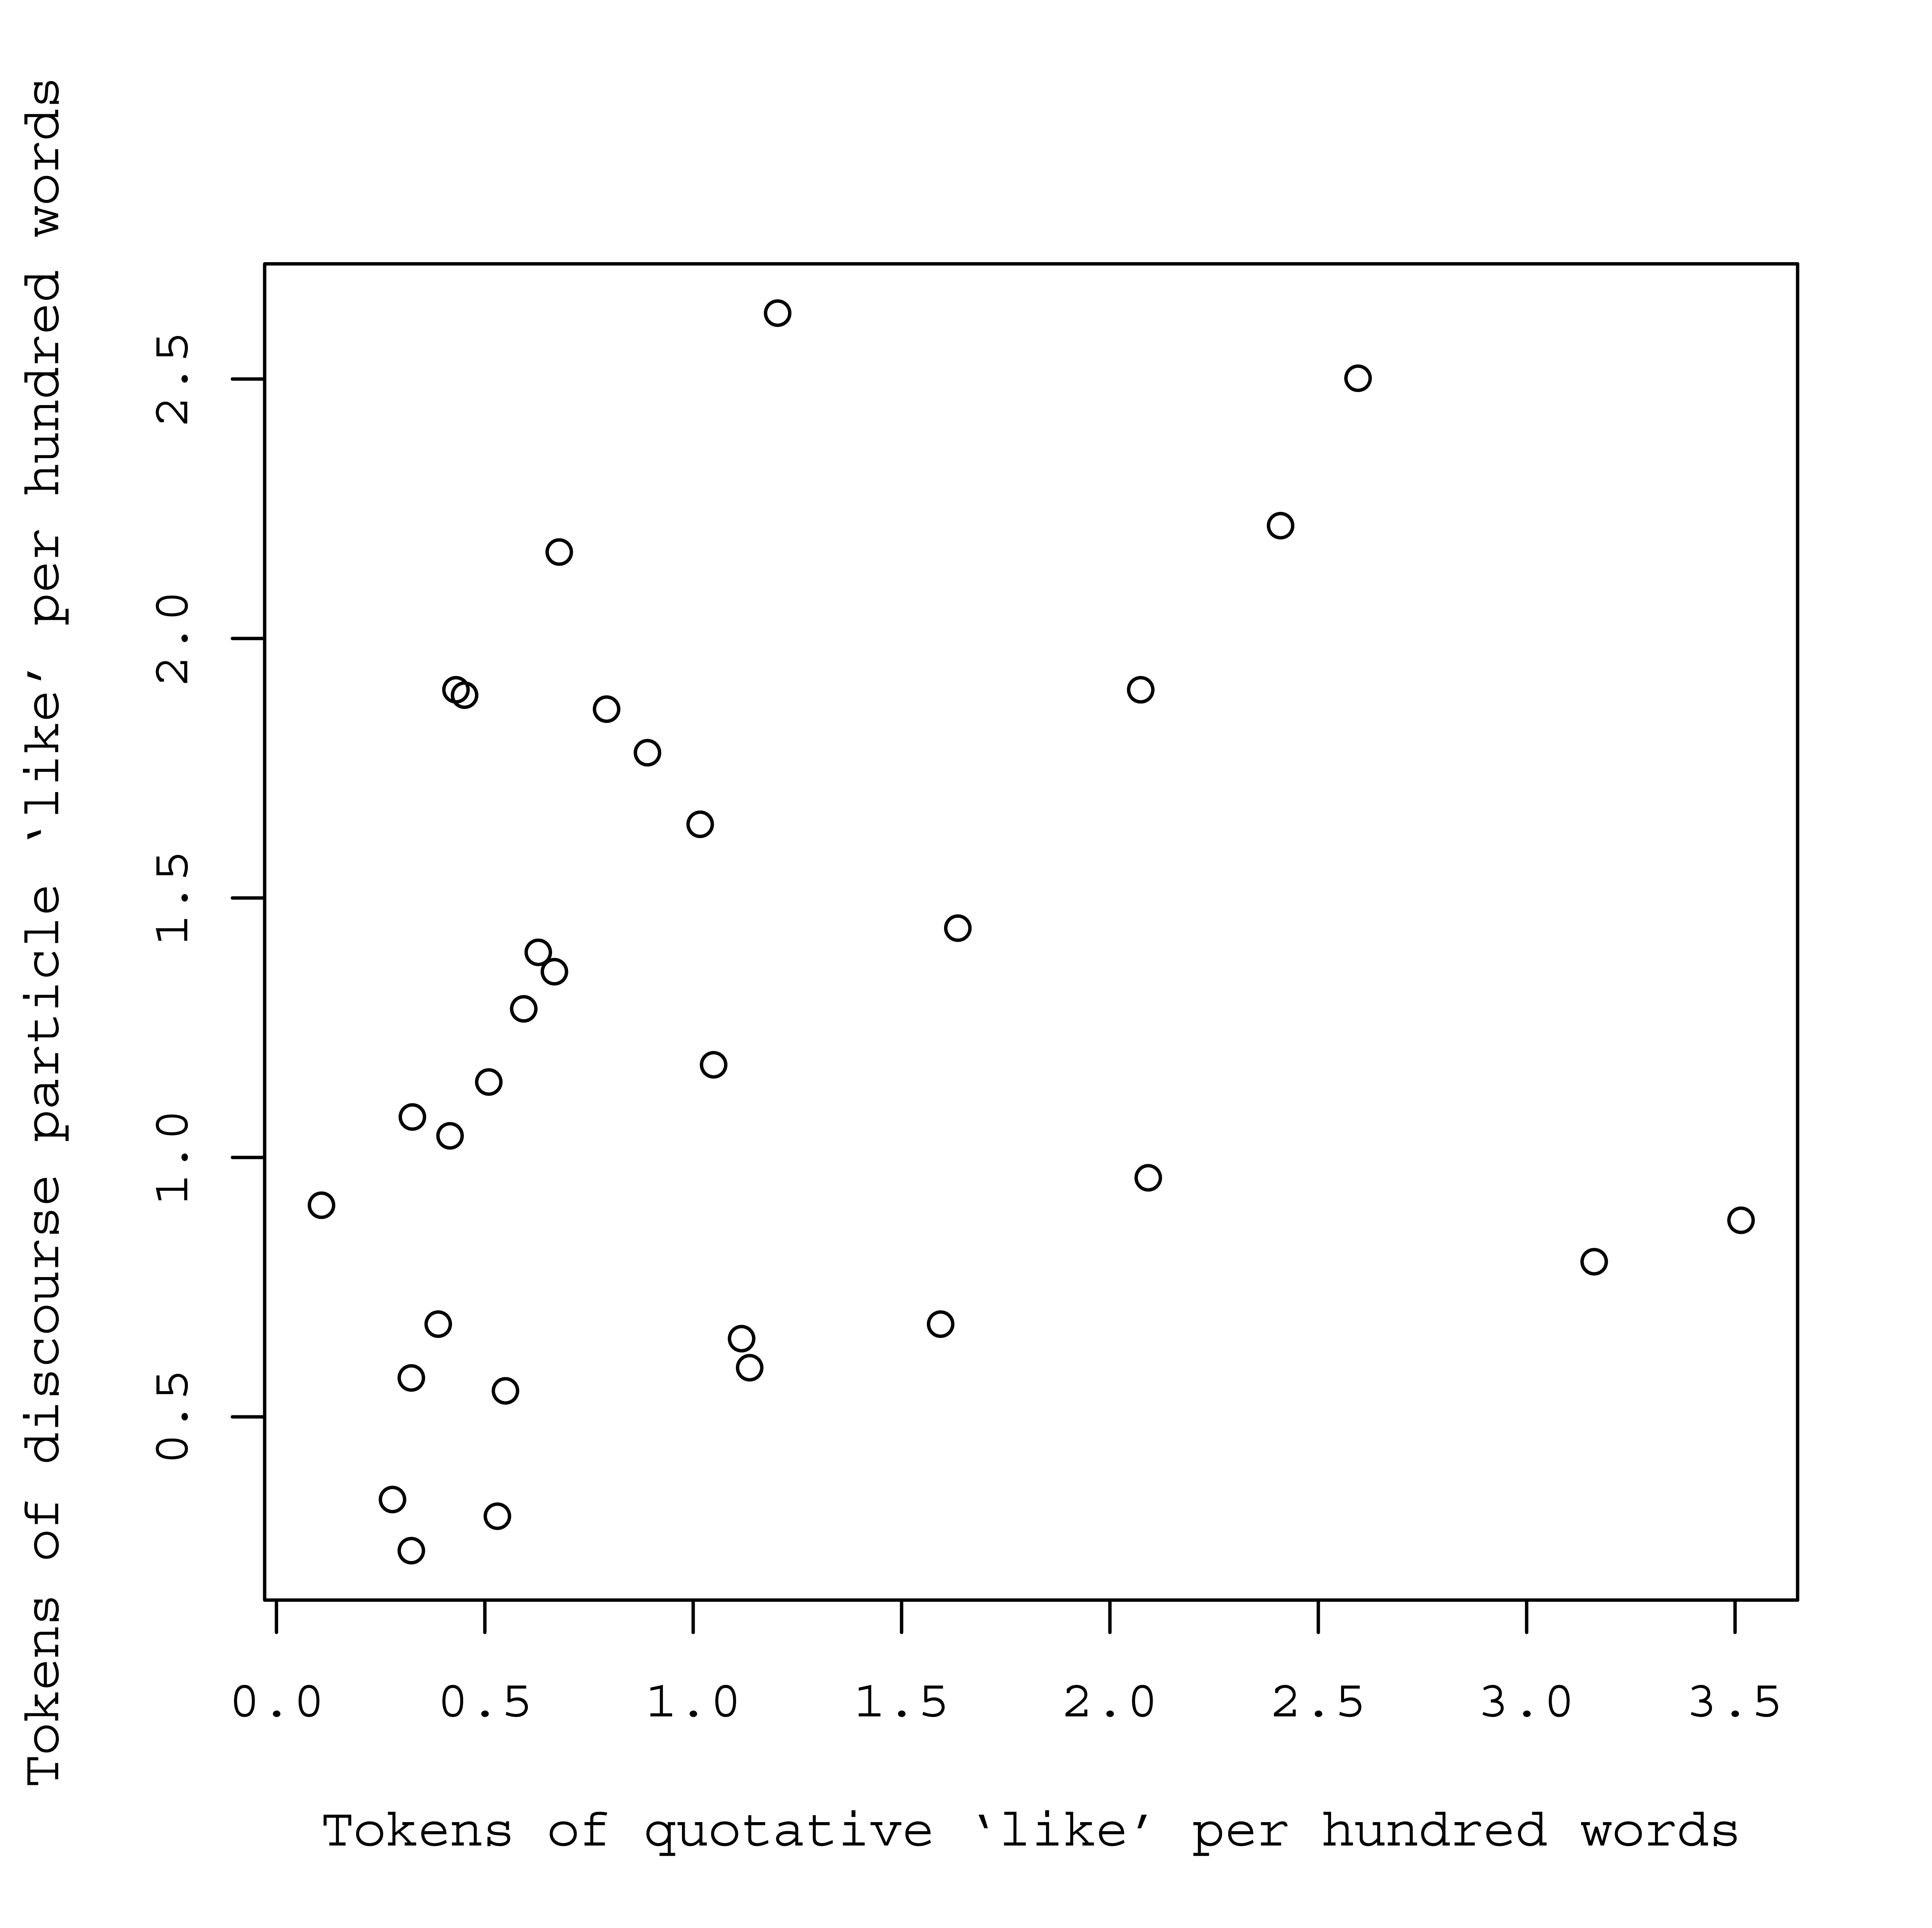
\includegraphics[width=5in]{images/freofuseCompare.jpg}
	\caption{Plot of the number of tokens of quotative \textit{like} and the number of tokens of discourse particle \textit{like} per hundred words produced.}
	\label{fig:ComparingQDP}
\end{figure}


%%%%%%%%%%%%%%%%%%%%%%%%%%%%%%

\section{Phonetic variation of \textit{like}}\label{sec:phoneticlike}

There is variation among the girls' realizations of \textit{like} in several respects: whether or not the /k/ is realised, the length and quality of the /l/, how diphthongal the vowel is, the vowel quality of the nucleus and offglide targets, the duration of the vowel, and the degree of glottalisation.  All of these factors were analysed in order to determine whether there was any fine-grained phonetic variation that patterned systematically with (a) whether or not a speaker was a CR girl and (b) the different functions of \textit{like}.  


The CR-NCR distinction at SGH was noticed prior to beginning acoustic phonetic analysis.  However, in order to determine whether this was an appropriate social distinction to include in the statistical analysis, I conducted a classification and regression tree (CART) analysis (see e.g., Breiman, Friedman, Olshen and Stone (1984)) predicting /k/ realisation before fitting the statistical model presented in Section \ref{sec:prodresults}.  Individuals grouped according to whether or not they ate lunch in the CR, which suggested that the CR-NCR distinction was in fact an appropriate social category to include in the model. \nocite{breimanetal1984}



\subsection{Methodology for acoustic phonetic analysis}\label{sec:phoneticmethod}


The various utterances of \textit{like} from the interviews were extracted automatically from the corpus using ONZEMiner \cite{onzeminer}.  Because of the particular functions chosen for analysis, the vast majority of tokens did not occur at phrase boundaries, did not carry primary stress, and were not the least stressed words in the sentence; only one token analysed occurred sentence-finally and carried primary stress.  

I aimed to conduct acoustic analysis on 30 tokens of \textit{like} for each girl.  Whenever possible, these 30 tokens were made up of 10 tokens of quotative \textit{like}, 10 tokens of the discourse particle, and 10 grammatical tokens.  The grammatical tokens were made up of a combination of lexical verbs and adverbs depending on what was present in the data.\footnote{Preliminary analysis provided evidence that the lexical verb and the adverb were phonetically similar to one another for a given speaker in terms of /k/ presence and the degree of diphthongisation.}  This, however, proved impossible for all girls due to low token numbers, and fewer than 30 tokens were analysed for some girls.  For girls with more than 10 tokens of a particular function of \textit{like}, the first 10 tokens extracted were analysed provided that they were unobscured by background noise.  The token distribution is shown in Table \ref{tab:tokensanalysed}.

  
%summary(noapproxtype.lab)
 %         approxadv        dm        dp   lexverb      prep     quote 
  %      0         0         0       292       104       100       239 
%> summary(CRtype.lab)
 %         approxadv        dm        dp   lexverb      prep     quote 
  %      0        22        58       160        48        49      119  
%> summary(NCRtype.lab)
 %         approxadv        dm        dp   lexverb      prep     quote 
  %      0        11        29       132        56        51       120 
      %  summary(noapprox$CR)
     %CR NCR 
  %0 376 359 
        
\begin{table}[htbp]
\caption{The distribution of analysed tokens of \textit{like} for CR and NCR groups.}
  \label{tab:tokensanalysed}
	 \begin{center}
		\begin{tabular}{lrrr}\lsptoprule
	
		& \sc cr 	&	 \sc ncr & \sc total \\
              
  \midrule
  
quotative & 119 & 120 & 239 \\
discourse particle & 160 & 132 & 292 \\
grammatical (lexical verb) & 48 & 56 & 104\\
grammatical (adverb) & 49  & 51 & 100 \\
grammatical (total) & 97 & 107 & 204 \\
total analysed      & 376 & 359 & 735 \\

\lspbottomrule
		\end{tabular}
	
	\end{center}
\end{table}

The final dataset included 104 tokens of the lexical verb and 100 tokens of the adverb, resulting in 204 tokens of traditionally grammatical functions.  There were 239 tokens of the quotative and 292 tokens of the discourse particle in the final dataset.  Of the 3159 tokens of \textit{like} initially extracted for the speakers analysed, 735 tokens (or roughly	23\% of the tokens extracted) were analysed using detailed acoustic analysis.\footnote{The percentage of tokens extracted that were analysed breaks down by function as follows: 30\% of quotative \textit{like} tokens extracted, 28\% of discourse particle tokens extracted, 60\% of lexical verb tokens extracted, 40\% of adverb tokens extracted.  If a greater number of tokens were analysed, it is possible that a larger number of factors would reach significance in an interaction with the social factor tested.}  Tokens masked by noise or made ambiguous from false starts were not included in the analysis.  

The unequal distribution and the low token numbers for some groups would pose a problem for an analysis of the smaller sub-groups (e.g., the Goths, the PCs).  The analysis presented here focuses on differences at the CR/NCR level, though individual speaker differences are discussed in Section \ref{theindividual}.   
%They were then assigned one of the categories (discourse particle, quotative, or grammatical) based on the grammatical function of the token.  

Phonetic features of the tokens were la\-belled in Praat text\-grids \cite{boersmaweenink} in a way that allowed the analysis to be conducted both on gradient and discrete measures.\footnote{A small subset of the data was checked for consistency by an independent phonetician.}  The bound\-aries be\-tween words were marked, as were the phoneme boundaries within the word \textit{like} and the nucleus and offglide boundaries of the diphthong; gradient measures such as segment duration and formant values could be tested and gradient measures such as whether or not the /k/ was present (i.e. there were no boundaries marked for the /k/) could also be tested.  Segmentation of this type is notoriously difficult because there are not clear acoustic boundaries between the segments \cite[142]{ladefoged2003}.  For consistency, the following methodological decisions were made:

\begin{enumerate}
	\item When preceded by a vowel, the first boundary of the /l/ was marked at the point where there was a noticeable dampening of the intensity in the waveform.  When preceded by a fricative or a released stop, the boundary was marked at the point where there was a noticeable increase in the amount of periodic energy or, if absent, when there was a noticeable decrease in the amount of aperiodic energy in the signal as evidenced in the waveform.  When preceded by a pause, the boundary was marked at the onset of voicing.  When following a nasal, it was marked where there was a noticeable change in F2 or, due to an increase in tongue contact, a sudden dampening of amplitude as evidenced in the waveform.
	\item The word boundary following the /k/ was marked after any evidence in the spectrogram and waveform of the /k/ release if the release was present.  Due to the difficulty of finding tokens of \textit{like} where the entire token was unobscured by other noises (e.g., someone else talking), I prioritised finding tokens that were clear in other parts of the signal rather than the release.  Therefore, I am not entirely confident about the segmentation following the release, so the duration of the release was not analysed.  When the release was not present, the boundary was marked at the onset of the following segment.  For example, if there was no closure period and the token was followed by a vowel other than \textipa{/i/} or \textipa{/I/}, formant transitions were used to identify the boundary.  There were no tokens followed by \textipa{/i/} that were analysed and for the eight tokens followed by \textipa{/I/}, other cues were used.  These cues included a transition in pitch and the point at which the vocal pulses are closer together after being further apart.
	\item The boundary between the /l/ and the vowel was marked at a point where there was an increase in amplitude visible in the waveform.  Because the amplitude was most often a gradual shift, the boundary was marked at the point just before a sharp rise in F1 toward the target of the following /ai/.
	\item The boundary between the vowel and the /k/ was marked at the point of closure or, in the case of frication and zero closure, at the point where aperiodic energy began.
	\item For tokens that were diphthongal (to any degree), the boundary between the nucleus and offglide was marked roughly at the half-way point in the transition between two steady states.  For completely monophthongal tokens, the boundary was marked at the halfway point of the vocalic portion.  This was done solely as a way to aid the automatic extraction of the labels; the durations of the nucleus and offglide were not analysed.
	
\end{enumerate}

\noindent Also marked were the targets of the nucleus, offglide, /l/, and /k/. The target of the nucleus was marked at the point where F1 was highest and, if there were multiple points where F1 was high, where F2 was lowest.  The target of the offglide was taken where F1 was lowest and F2 was highest but before a sudden drop in F1 that preceded the /k/ closure, if there was one.  The /l/ target was taken midway between the influence of the preceding sound and the onset of the vowel at a point where F2 was visible.\footnote{This measure was initially intended to be used to calculate /l/ vocalisation.  However, I was unhappy with this measurement (see e.g., \citeasnoun{halllewfix2012}).  Additionally, I was surprised by the large number of tokens where /l/ was not present or where it was so short that F2 could not be reliably identified in the spectrogram.  Therefore, the /l/ target was not analysed.}  The /k/ target was taken at the point of the offglide where F3 was lowest. 

A three-way distinction of glottalisation of the vowel (not glottalised, mid-glottalisation, and full glottalisation) was also made.  This was based on a judgment of the amount of irregularity in the intervals between the pulses of the vocal folds, as evidenced through both pulses in the waveform and striations in the spectrogram.  The categories full and not glottalised were used when glottalisation (or the lack of it) was easily identifiable: a token was marked as not glottalised if there were evenly-spaced pulses in the token even when compared to the surrounding speech produced by the same speaker; a token was marked as fully glottalised if the intervals between pulses were considerably larger in some portion of the token than in another part of the token or the speech produced by that speaker surrounding the token.\footnote{A distinction in the duration of the glottalised portion of the token was not made.}  The third category, mid-glottalisation, was used when assignment to one of the other two categories was not clear.  In addition to tokens with creaky voice, tokens with glottal stops were marked as fully glottal, following work by Docherty and Foulkes who found that creaky voice was identified as a glottal stop during auditory analysis \cite{dochertyfoulkes1999}.  Additionally, all tokens that may have been marked as containing a glottal stop had an increasing amount of glottalisation preceding the stop, making it difficult to distinguish these tokens from those with creaky voice at the end of the vocalic period and no glottal stop.  Glottalisation in different parts of the token were not differentiated from one another.

%Through marking the segment boundaries and giving a different label to each segment within a token, the presence or absence of a segment is essentially also encoded into each of the textgrids.  The greatest amount of variation of presence or absence was found in terms of the /k/  Therefore, whether a /k/ was present in any given token  

Regarding the /k/, the boundaries between the vowel, closure, and release were marked.  For tokens where there was no closure period but there was a release, the boundary was marked at the point where aperiodic energy began in the signal.\footnote{The burst was not coded but would be an interesting avenue for future work.}  A /k/ was marked as dropped if it could not be heard during auditory analysis and one of the following applied:

\begin{enumerate}
	\item The token was followed by a continuous segment (e.g., a vowel) and there was no period of closure or release.
	\item The token was followed by a stop and there was no evidence of a velar closure (e.g., a velar stop); there was complete assimilation to the place of the following segment.\footnote{It is important to bear in mind that tokens where the /k/ was dropped and were followed by a stop were in the minority of the tokens analysed; 26 tokens were followed by a stop and labelled as having the /k/ not realised, compared with the 58 tokens that were followed by a stop and had the /k/ realised.  Additionally, the 26 tokens followed by a stop where the /k/ was marked as dropped were not distributed across CR and NCR girls in a way that could be interpreted as the explanation for the results presented in this chapter; eight were tokens of the discourse particle and two were tokens of the quotative produced by CR girls and six were tokens of the discourse particle and one a token of the quotative produced by NCR girls.}  For the 84 tokens that were followed by a stop, the transitions of F2 and the presence of a velar pinch \cite[89]{harringtoncassidy1999} were used to determine whether assimilation had taken place.
	\item The token was followed by a pause and the formants from the token of \textit{like} trail off gradually, as they do with pre-pausal vowels.
	\item One of the above applied and the token was glottalised, in which case the token was marked as glottalised but not having the /k/ realised.
\end{enumerate}

\noindent Although glottalisation and glottal stops are often treated as a particular realisation of /k/ \cite{lavoie2002}, it was marked separately from /k/ realisation for this study because glottalised tokens were sometimes produced with a clear closure and release of the /k/.  Additionally, marking glottalisation and /k/ realisation allowed them to be tested both as separate factors or as a single variable once combined; treating them as a single factor during the phonetic analysis would only permit the latter. 

To demonstrate how the textgrids were marked, examples are shown in Figures \ref{fig:469santra}-\ref{fig:brenda15}.

\begin{figure}
	\centering
		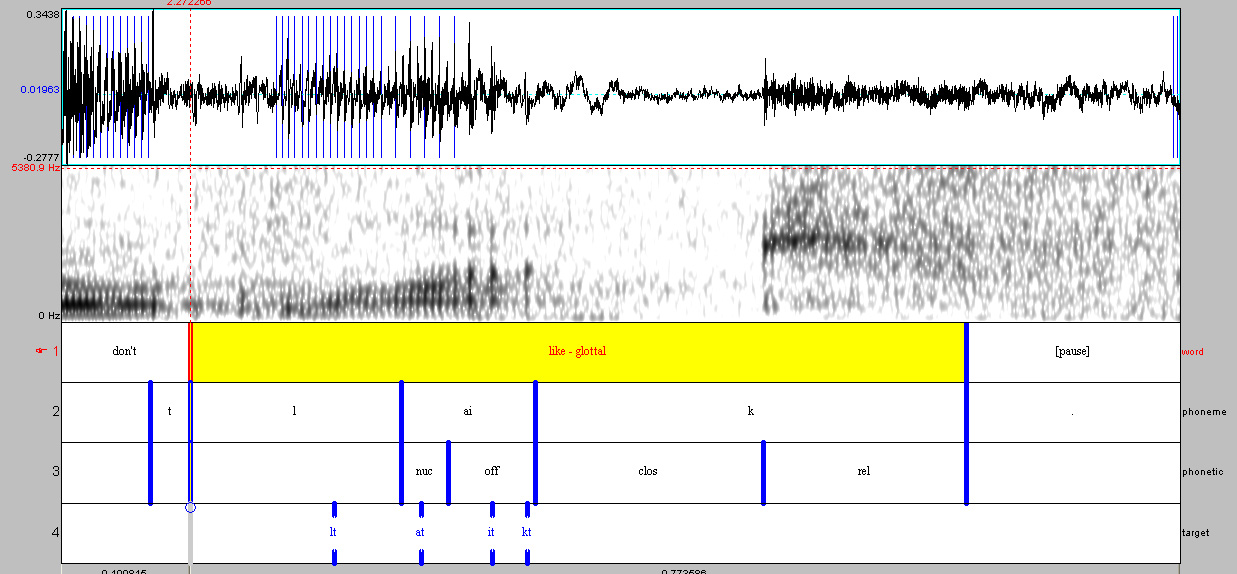
\includegraphics[width=5in]{images/469santra.jpg}
		\caption{Lexical verb \textit{like} from Santra (The Goths).  /l/ present, diph\-thongal vowel, glottalised,  /k/ released, preceded by stop, followed by pause.} 
	\label{fig:469santra}
\end{figure}

\begin{figure}
	\centering
		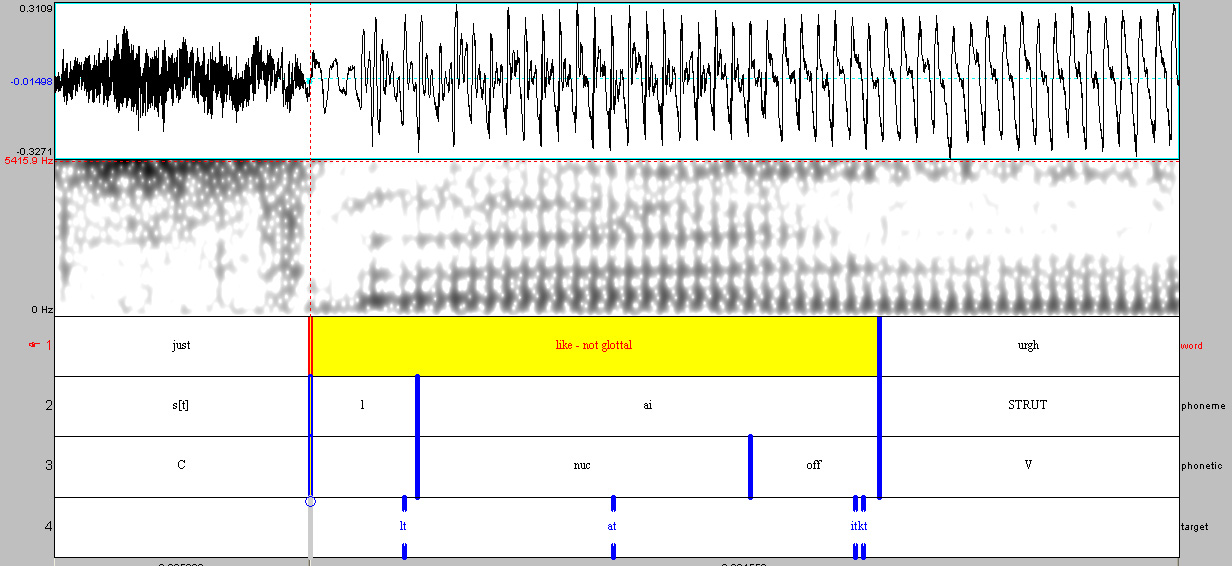
\includegraphics[width=5in]{images/patricia74.jpg}
	\caption{Quotative \textit{like} from Patricia (Sporty Girls). /l/ present, diph\-thongal vowel, not glottalised, /k/ absent, preceded by fricative, followed by vowel.}
	\label{fig:patricia74}
\end{figure}

\begin{figure}
	\centering
		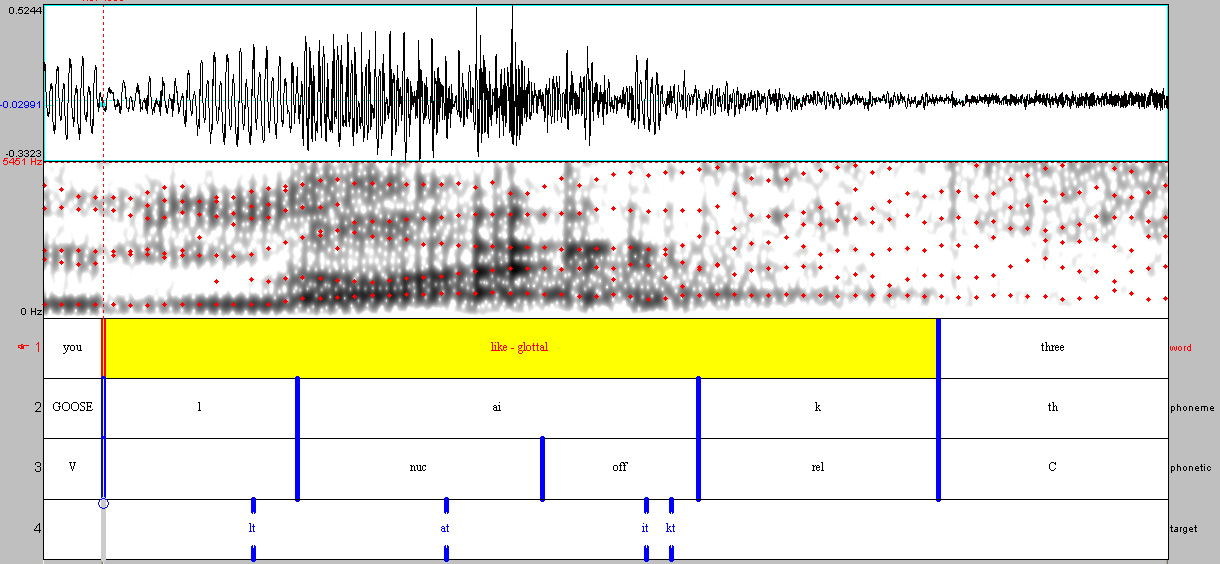
\includegraphics[width=5in]{images/barbara19.jpg}
	\caption{Adverbial \textit{like} from Barbara (The Relaxed Group). /l/ pre\-sent, diph\-thongal vowel, glottalised, fricated /k/, preceded by vowel, followed by fricative.}
	\label{fig:barbara19}
\end{figure}

\begin{figure}
	\centering
		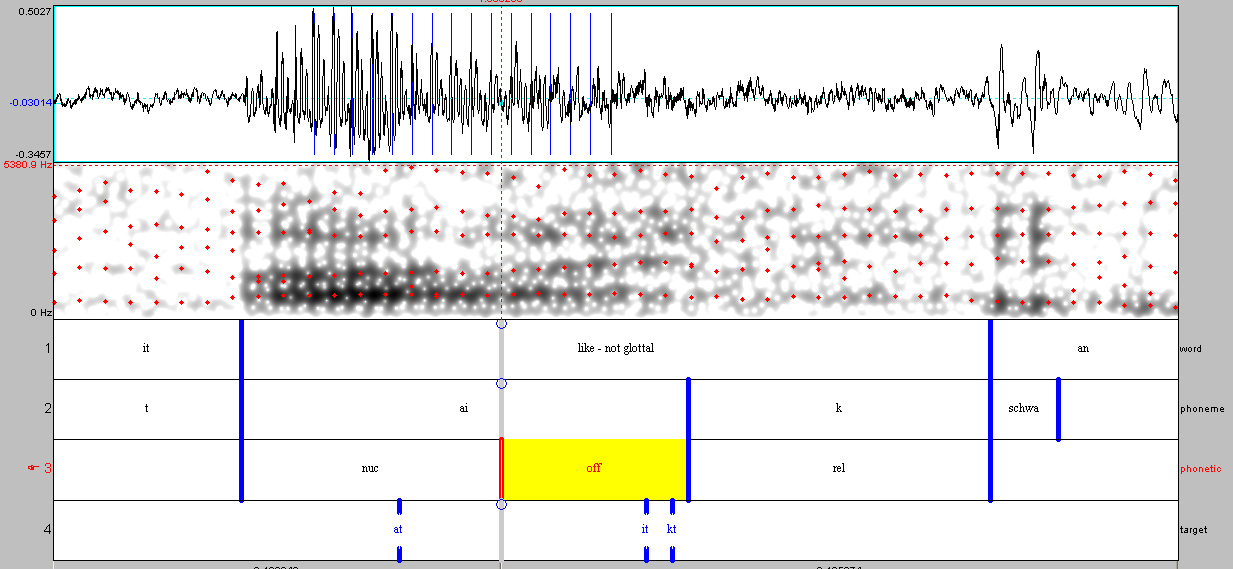
\includegraphics[width=5in]{images/jane37.jpg}
	\caption{Adverbial \textit{like} from Jane (The BBs).  /l/ absent, diphthongal vowel, not glottalised, fricated /k/, preceded by stop, followed by vowel.}
	\label{fig:jane37}
\end{figure}

\begin{figure}
	\centering
		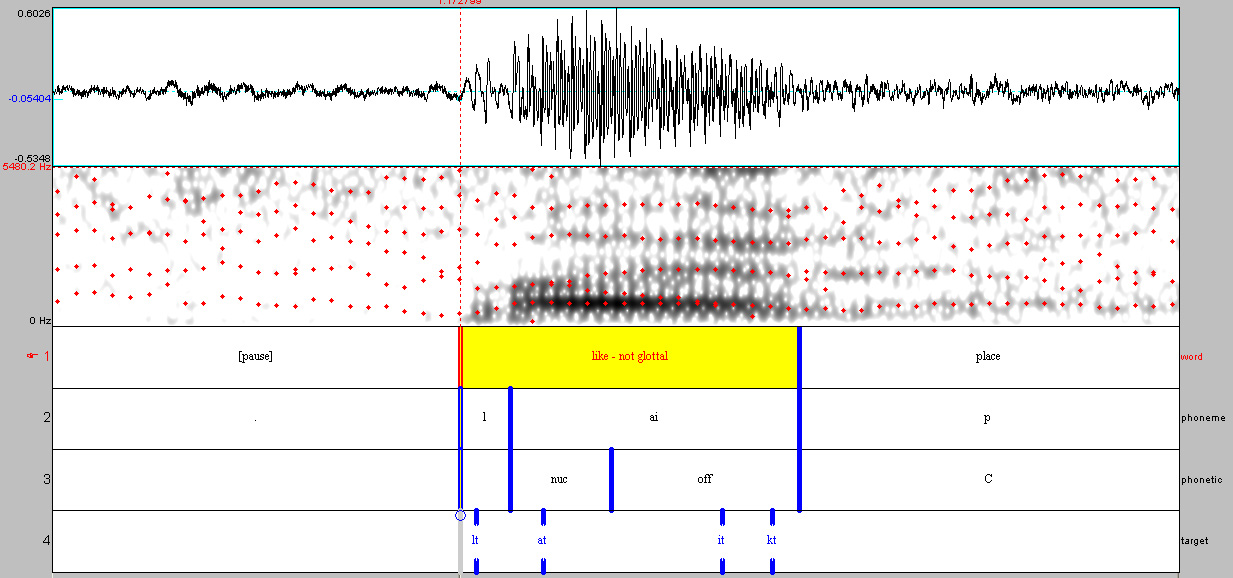
\includegraphics[width=5in]{images/rochelle2.jpg}
	\caption{Discourse particle \textit{like} from Rochelle (Rochelle's Group).  /l/ present, diphthongal vowel, not glottalised, /k/ absent, preceded by pause, followed by stop.}
	\label{fig:rochelle2}
\end{figure}

\begin{figure}
	\centering
		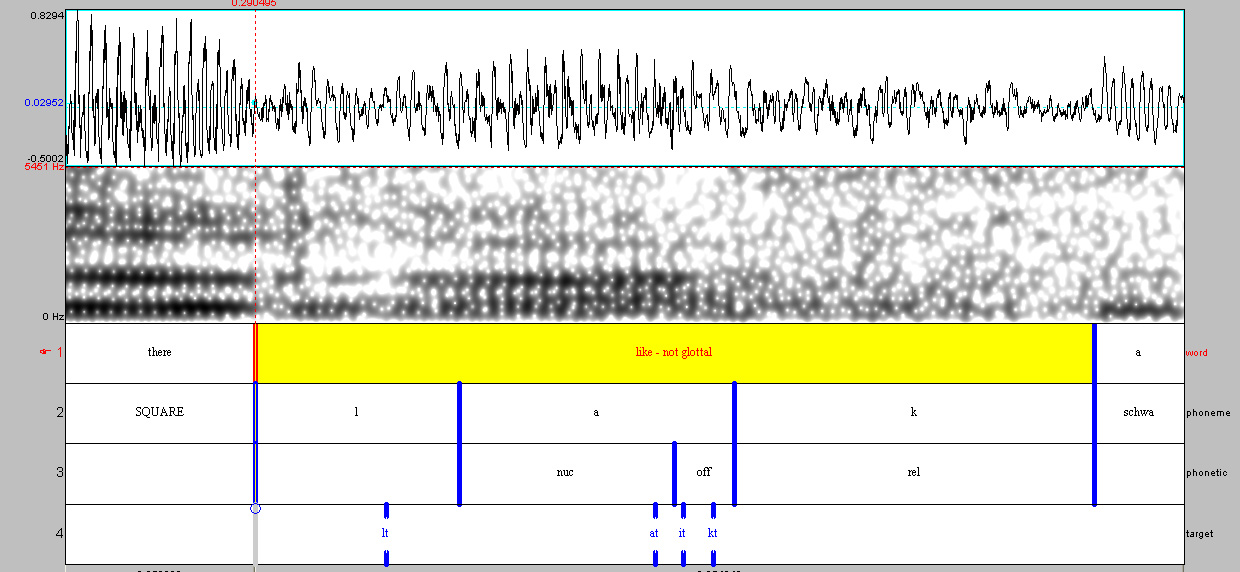
\includegraphics[width=5in]{images/brenda15.jpg}
	\caption{Discourse particle \textit{like} from Marama (The Pasifika Group).  /l/ present, monophthongal vowel, not glottalised, fricated /k/, preceded by vowel, followed by vowel.}
	\label{fig:brenda15}
\end{figure}





Tokens that were followed by a velar consonant were not included in the analysis.  The preceding and following pho\-nemes were marked in the text\-grids, with an additional level distinguishing only between vowels, consonants, and pauses.  Pauses were labelled as such when a phone did not immediately follow a token of \textit{like}.  Voiced continuants, such as \textipa{/l/}, were labelled as consonants.  For counts of phonetic features in the raw data, refer to Appendix \ref{appen:proddata}.  


After completion, the textgrids were converted into files that could be read by Emu \cite{emu}.  In Emu, formant traces were corrected by hand.  The formant values were extracted automatically along with other encoded information (e.g., segment duration and whether the token contained a released /k/) using a tailor-made library in the statistical software package, R (R Development Core Team 2007).  

Target values of the nucleus and offglide were converted from Hertz to Bark using the equation posited by \citeasnoun{traunmuller1990} and the Euclidean distance of a token's vowel was calculated using these F1 and F2 values of the nucleus and offglide targets.\footnote{For formant values, the Bark scale was used instead of Hertz because it is a better reflection of how formants at the different frequencies are perceived by human listeners.  For example, a shift in F1 is perceived as greater than a shift in F2 of the same amount in Hertz.}  A completely monophthongal vowel would have a Euclidean distance value of zero, whereas a value of five Bark would be extremely diphthongal. Euclidean distance can therefore be viewed as a gradient measure of how diphthongal a vowel is; the greater the Euclidean distance, the more diphthongal the token. 
\nocite{r}


A token's pitch was extracted automatically at 10ms intervals throughout the vowel using the AMDF method in Emu.  The mean pitch for each token was calculated from the extracted values.  Pitch measurements at the nucleus and offglide targets were also extracted and they were used to determine whether a token had a steady or moving intonation.  Tokens with a transition of 10Hz or more were labelled as `moving'.  Due to limits on time, pitch contours were not corrected by hand in Emu, so results regarding pitch should be viewed with some caution.  In order to keep them from biasing results, tokens with a mean pitch that was over two standard deviations away from the mean were assigned the pitch value at the cutoff point. 



\subsection{Results}\label{sec:prodresults}
%Preliminary analysis revealed that quotative \textit{like} behaved differently from the other functions of \textit{like} with a number of different phonetic variables.  An analysis of these factors will be presented in Section \ref{section:quotenonquote}.  Additional differences were found between discourse particle \textit{like} and grammatical functions of \textit{like}.  These differences will be discussed in Section \ref{discpgram}. 

The raw data is presented in Appendix \ref{appen:proddata}, with the numbers of different tokens with each phonetic characteristic listed according to whether the speaker was a CR or a NCR girl.  Because each of the factors is best understood within the context of all of the other factors, the results are presented in this chapter within the context of statistical models.

In order to test the relationship between the function of \textit{like} and numerous phonetic factors, three mixed effects models were fit to the production data.  Like simple linear and logistic regression models, a mixed effects model allows for numerous predicting factors to be included in a single model.  Significance levels and the degree of each effect are calculated whilst keeping the other factors constant.  This effectively takes into consideration the influence of the other variables when investigating a particular factor.  For example, assume /k/ realisation only patterns systematically with following environment (e.g., it is more likely to be realised when followed by a vowel) and following environment predicts the dependent variable being tested.  This could lead to /k/ realisation appearing to be a predicting factor of the dependent variable if following environment is not included in the model. 

Another benefit of using mixed effects models is that in addition to allowing the inclusion of fixed effects, such as phonetic and social factors that can systematically predict the form of the dependent variable, random (non-generalisable) effects can be included \cite[263-326]{baayen2008}.    Random effects can be speaker-specific effects or, in experimental work, stimuli-specific effects.  For example, in an analysis of reaction time, some participants may be faster than others.  If the researcher wants to examine predicting factors above and beyond this participant-specific effect, they could include the participant as a random effect in the model.   Including the speaker as a random effect reduces the risk that a single individual will bias results.\footnote{The random effects included in these models were random intercepts.  Random slopes were tested but did not change the reported trends, so the simpler models are included.} 

The first model presented in this chapter compares realisations of quotative \textit{like} to grammatical functions of \textit{like}.  The second compares realisations of quotative \textit{like} to discourse particle \textit{like}, and the third compares realisations of the discourse particle to grammatical functions of \textit{like}.  A summary of results of all three models can be found at the end of the section in Table \ref{tab:sumprodresults}. 

\subsubsection{Model 1: Grammatical and quotative \textit{like}}

Using R, a mixed effects model was fit to the data comparing the quotative with grammatical functions of \textit{like}, modeling the likelihood that the token was the quotative.  The speaker was included as a random intercept.    Before fitting the model, I assumed an alpha level of 0.05 as the threshold for statistical significance.  

A number of factors were tested as potential effects in the model, including vowel duration, preceding and following environment, the different calculations of pitch (mean pitch and steady versus moving pitch), and the speech rate (calculated as syllables per second in both the 5 seconds and 20 seconds of speech surrounding a token).\footnote{Only speech that was produced by the same speaker who produced the tokens was used to calculate speech rate.}  Also tested was whether the speaker was a girl who ate lunch in the CR, whether the /k/ and /l/ were realised, the duration of the closure period of the /k/, and linear as well as non-linear distributions of the Euclidean distance of a token's vowel.  In order to determine whether the probability of a speaker using quotative \textit{like} played a role, tested in the model were interactions between phonetic factors and the two calculations of an individual's use of \textit{like}: the number of tokens of quotative \textit{like} per hundred words produced by that speaker and the percentage of all quotatives produced by an individual that were quotative \textit{like}.\footnote{Both calculations were tested to determine whether they had any power in predicting the relationship between function and phonetic form, both to inform future work in this area and because they have different theoretical implications.  The number of tokens of quotative \textit{like} per hundred words failed to reach significance in the model when in place of the second calculation (p$>$0.1).}  Also tested was the number of tokens of the discourse particle observed for each girl per hundred words produced.  Factors reaching significance were included as fixed effects in the model.  Also included in the first model are two factors that are approaching significance (p$<$0.06).  These are included in the model in order to account for the variation they appear to be predicting (thereby creating a better fit model).  The model's fixed effects and their coefficients for the test variables are shown in Table \ref{qgcoeffProd}, and the control variables from the model are shown in Table \ref{qgcoeffProd-control}.\footnote{The final model was also fit only to data from girls who had ten or more quotatives (see Table \ref{tab:percentlike}).  All factors reached the same level of significance as in the model reported here.  Similarly, the final model was fit first only comparing the quotative with the lexical verb and then comparing it with the adverb.  All effects reached significance and were in the same direction as the model presented here with the exception of the value of F2, which did not reach significance in either of the models.  This provides additional evidence that the lexical verb and the adverb were similar phonetically.}  The estimated scale parameter of a model is a measure of how much of the actual variance in the data can be accounted for by the model.  Ideally, it is close to 1.  The estimated scale parameter for this model is 1.030892, which indicates that it is a good fit.
 

% latex table generated in R 2.6.1 by xtable 1.5-2 package
% Thu Aug 14 10:32:25 2008
\begin{table}[ht]
\begin{center}
\begin{tabular}{lrrrr}
  \hline
 & Estimate & Std. Error & z value& Pr($>$$|$z$|$) \\
  \hline  
  
(Intercept)      &  0.3366 &  0.68  & 0.50 & 0.6198 \\
DIPH             &  -0.4367  & 0.13  & -3.46 & 0.0005 \\
PITCH            &  0.0072 &  0.00  &  3.51 & 0.0005 \\
LV DURATION      &  -2.2391 &  0.59  & -3.81 & 0.0001 \\
   \hline
\end{tabular}
\caption{Coefficients of fixed effects for Model 1, comparing the quotative with grammatical functions of \textit{like}.}
\label{qgcoeffProd}
\end{center}
\end{table}


\begin{table}[ht]
\begin{center}
\begin{tabular}{lrrrr}
  \hline
 & Estimate & Std. Error & z value& Pr($>$$|$z$|$) \\
  \hline  
preceded by pause        &  -0.8199  & 0.87 & -0.94 & 0.3482 \\ 
preceded by fricative  		& 1.7364 &  0.28  & 6.21 & $<$0.0001 \\
followed by pause         &  0.8526 &  0.52  & 1.64 & 0.1015 \\
followed by V             &  -0.1981 &  0.42 & -0.47 & 0.6379 \\
followed by sibilant        & -1.8554  & 0.65  & -2.87 & 0.0041 \\
followed by nasal           & -1.0028  & 0.55  & -1.81 & 0.0697 \\
followed by other voiceless  & -1.8175 &  0.51 & -3.53 & 0.0004 \\
followed by other voiced     & -3.1986 &  0.57 & -5.65 & $<$0.0001 \\
   \hline
\end{tabular}
\caption{Coefficients of control variables for Model 1, comparing the quotative with grammatical functions of \textit{like}.}
\label{qgcoeffProd-control}
\end{center}
\end{table}



Fixed effects in the model include the preceding and following environment, the Euclidean distance between F1 and F2 of the nucleus and offglide as a measure of how diphthongal the token's vowel was (DIPH), the mean pitch (PITCH), and the ratio of /l/ to vowel duration (LV DURATION).  

The defaults of the model are that the token was preceded by something other than a fricative or a pause and was followed by a consonant (followed by C).  For continuous factors, the model assumes a value of zero, even when this value is not present in the data.  Therefore, the model assumes as a default that the vowel was completely monophthongal (DIPH = 0) and that the /l/ to vowel duration ratio was zero (LV DURATION = 0), both of which are values that were observed in the data.  Tokens with an /l/ to vowel duration ratio of zero were tokens where there was no acoustic evidence of an /l/; the /l/ was dropped.  The intercept's estimate given in Table \ref{qgcoeffProd} is the likelihood in log odds that a token with the default characteristics was quotative \textit{like}.  To determine the log odds for tokens that do not match the default criteria, the estimate for binary factors must be added to the default intercept of the model.  For example, to determine the likelihood that a token was quotative \textit{like} if it had the default characteristics except that it was followed by a pause, the estimate for tokens followed by pauses (-0.8199) would be added to the estimated intercept (0.3366).    For continuous factors, such as Euclidean distance, the product of the factor's coefficient and the token's Euclidean distance is added to the estimated coefficient of the intercept.  In calculating log odds of factors for the graphs presented in this chapter, the mean values of continuous factors were used as defaults.

Prior to running the final model, the different preceding environments were run as separate factors in the factor group for the preceding environment.\footnote{First, the different phonemes which preceded each token were treated as factors.  They were then divided depending on voicing and on whether they were continuous.  Whether a token was continuous did not significantly predict the function of \textit{like}.  Voiceless tokens were less likely to precede the quotative than the grammatical function (p$<$0.05), but there is no interaction between voicing and whether the preceding environment was a fricative.  This makes it unlikely that the shorter /l/ to vowel duration ratio associated with the quotative was due to identifying portions of the /l/ that were voiceless (as a result of coarticulation) as the preceding segment.}  They appeared to clump according to whether they were a fricative, a pause, or something else.  Therefore, the factor group for the preceding environment that was included in the final model had this three-way distinction.  As indicated by the positive coefficient in Table \ref{qgcoeffProd}, tokens that were preceded by a fricative were significantly more likely to be the quotative than a grammatical function when compared to tokens that were preceded by a segment that was non-fricated (p$<$0.0001).  Although there was not a significant difference between tokens that were preceded by a pause and by a non-fricated segment, these factors were not collapsed into a single factor in order to maintain consistency across the different production models.

For the factor group of following environment, the model was first tested with each phoneme listed as a separate factor (e.g., /f/, /b/, pause).  The following environment was divided into seven discrete factors: followed by an approximant, followed by a pause, a vowel, a sibilant, a nasal, by some other segment that was voiceless, and by some other segment that was voiced.  The preceding environment was divided into three discrete factors: preceded by a pause, preceded by a fricative, and preceded by anything else.  The model held the fixed effect of following environment constant when testing the other factors, so the predicted effect of other factors was independent from following environment.  

A token was significantly less likely to be quotative \textit{like} if it was more diphthongal (p$<$0.001).  The higher the Euclidean distance of a vowel, the less likely it was to be the quotative. This was a continuous factor and its relationship with the function of \textit{like} was also continuous; tokens with vowels that were more diphthongal were more likely to be a grammatical function of \textit{like}.   


A vowel's mean pitch also significantly predicted whether or not a token was the quotative.  The higher the mean pitch, the more likely it was that the token was quotative \textit{like} as opposed to a traditionally grammatical function of \textit{like} (p$<$0.001).  This is likely related to the prosodic position in a sentence of the different types of \textit{like}.  Though both lexical verb \textit{like} and quotative \textit{like} function as verbs, their syntactic properties differ, affecting their position in a sentence.  Impressionistically, lexical verb \textit{like} seemed to be produced in conjunction with a dip in the intonation contour, whereas quotative \textit{like} rarely was and was sometimes part of a rising contour that raised more steeply after the verb.  

Tokens with a larger /l/ to vowel ratio have a longer /l/ duration relative to the duration of the vowel.  These tokens with a relatively long /l/ were significantly less likely to be quotative \textit{like} than a grammatical function of \textit{like} (p$=$0.0001).  Though measures of speech rate failed to reach significance in differentiating between the functions of \textit{like}, using the ratio of /l/ to vowel duration helped to normalise the duration of /l/ across different rates of speech.  That the ratio reached significance in the model suggests that the relationship between /l/ duration and function of \textit{like} was not an artefact of different speech rates across the different functions.    



\subsubsection{Model 2: Quotative and discourse particle \textit{like}}

A mixed effects model comparing tokens of the quotative with tokens of the discourse particle was fit to the data, modeling the likelihood that a particular token of \textit{like} was the quotative.    As with the first model, speaker was included as a random effect.  The same factors as tested in model 1 were tested in model 2.  Only those reaching significance were included in the model.    These included how diphthongal the token was, the ratio of /l/ to vowel duration, the mean pitch of the token, and the preceding and following environment as described for the previous model.  Also reaching significance in the model was an interaction between whether or not the /k/ was dropped and whether the girl was in a group who ate lunch in the CR.  Speech rate, frequency of use of quotative and discourse particle \textit{like}, and whether the token had a steady intonation contour failed to reach significance and were not included in the model.  The coefficient table for the production model is shown in Table \ref{qdpcoeffProd}.  
 
  

% latex table generated in R 2.6.1 by xtable 1.5-2 package
% Thu Aug 14 09:54:29 2008
\begin{table}[ht]
\begin{center}
\begin{tabular}{lrrrr}
  \hline
 & Estimate & Std. Error & z value& Pr($>$$|$z$|$) \\
  \hline

(Intercept)   &  -0.4093 &  0.56  & -0.735 & 0.4626 \\
  DIPH        &  -0.4671 &  0.11  & -4.212 &  $<$0.0001 \\
  PITCH       &  0.0079  & 0.00   & 4.501  & $<$0.0001 \\
  LV DURATION &  -1.4819 &  0.49  & -3.024 & 0.0025 \\
  K-CLOS=N    &  -0.9035 &  0.30 & -2.987 & 0.0028 \\
  GROUP=NCR   &  -0.5364 &  0.34  & -1.560 & 0.1187 \\
  K-CLOS=N:GROUP=NCR  &  1.3050  & 0.44  & 2.97 & 0.0029 \\

   \hline
\end{tabular}
\caption{Coefficients of fixed effects for Model 2, comparing the quotative with the discourse particle.}
\label{qdpcoeffProd}
\end{center}
\end{table}
  


 
% latex table generated in R 2.6.1 by xtable 1.5-2 package
% Thu Aug 14 09:54:29 2008
\begin{table}[ht]
\begin{center}
\begin{tabular}{lrrrr}
  \hline
 & Estimate & Std. Error & z value& Pr($>$$|$z$|$) \\
  \hline
  preceded by pause     &  -2.8558 &  0.76 & -3.78 & 0.0002 \\
  preceded by fricative  &  0.8261  & 0.22 &   3.78 & 0.0002 \\
  followed by pause     &  0.0618  & 0.33  & 0.19 & 0.8516 \\
  followed by V         &  0.4689  & 0.32  & 1.45 &  0.1470  \\
  followed by sibilant  & -0.4713 & 0.59  & -0.80 &  0.4253 \\
	followed by nasal   & 0.3668   & 0.48  & 0.76 &  0.4475 \\
	followed by other voiceless  & -0.6591 &  0.42 & -1.56 & 0.1179 \\
	followed by other voiced   & -1.7862  & 0.51 & -3.50 & 0.0005 \\   
	
	\hline
\end{tabular}
\caption{Coefficients of control variables for Model 2, comparing the quotative with the discourse particle.}
\label{qdpcoeffProd-control}
\end{center}
\end{table}


  
A token was less likely to be a quotative if preceded by a pause than if preceded by a fricative (p$<$0.0001) or any other segment (p$<$0.001).   A token was more likely to be a quotative if preceded by a fricative than if preceded by any other segment (p$<$0.001).

A token's Euclidean distance also predicts the function of a token.  A token was significantly more likely to be quotative \textit{like} if it was more monophthongal (p$<$0.0001), as indicated by the negative coefficient value.  This is also similar to results from model 1.  

As with the first model, a token with a higher mean pitch was more likely to be quotative \textit{like} (p$<$0.0001).  Again, this is likely related to the words' prosodic position in a sentence.  Tokens of quotative \textit{like} were often followed by reported speech in a very high pitch, and the token of quotative \textit{like} itself rarely had the lowest pitch in the phrase.  Discourse particle \textit{like}, on the other hand, was produced in conjunction with a dip in the intonation contour.  It could have a very low pitch and was often produced with a creaky quality.

As in model 1, a token with a long /l/ duration relative to its vowel duration was less likely to be quotative \textit{like} than to be discourse particle \textit{like} (p$<$0.01).  This provides evidence that quotative \textit{like} had a shorter /l/ duration, regardless of speech rate.  Similar results were found in model 1, suggesting that quotative \textit{like} was most likely to have a shorter duration ratio, regardless of the non-quotative function with which it was paired.


The model includes a significant interaction between whether the /k/ in a token was realised or not and whether the girl who produced the token was a CR girl or not (p$<$0.01).\footnote{The interaction remains significant if the duration of the /k/ closure is included in the model in place of the discrete measure of whether or not the /k/ was realised.  Because the effect appeared to be carried entirely by the tokens where the closure duration was equal to zero as opposed to all other closure durations, the discrete measure was used in the model.}  A token where the /k/ was dropped was more likely to be quotative \textit{like} if produced by a CR girl, but less likely to be quotative \textit{like} if produced by a NCR girl.\footnote{The significance level presented here is for the interaction between CR and /k/ realisation.  Separate models fit first to the CR girls' data and then to the NCR girls' data, reveal that while the trend with /k/ realisation is significant for the CR girls (p$<$0.05), it is not significant for the NCR girls (p$>$0.7).  The arguments presented in this chapter are based on the opposite trends found for the two groups, which is why the interaction's significance level and coefficient are the focus of this discussion.}  This interaction, shown in Figure \ref{fig:kCR-qdp}, was independent of following environment, as following environment was included as a fixed effect in the model.  It seems there were not only differences in pronunciation between the different types of \textit{like} but that different social groups had different realisations for the different functions of \textit{like}.  


\begin{figure}
	\centering
		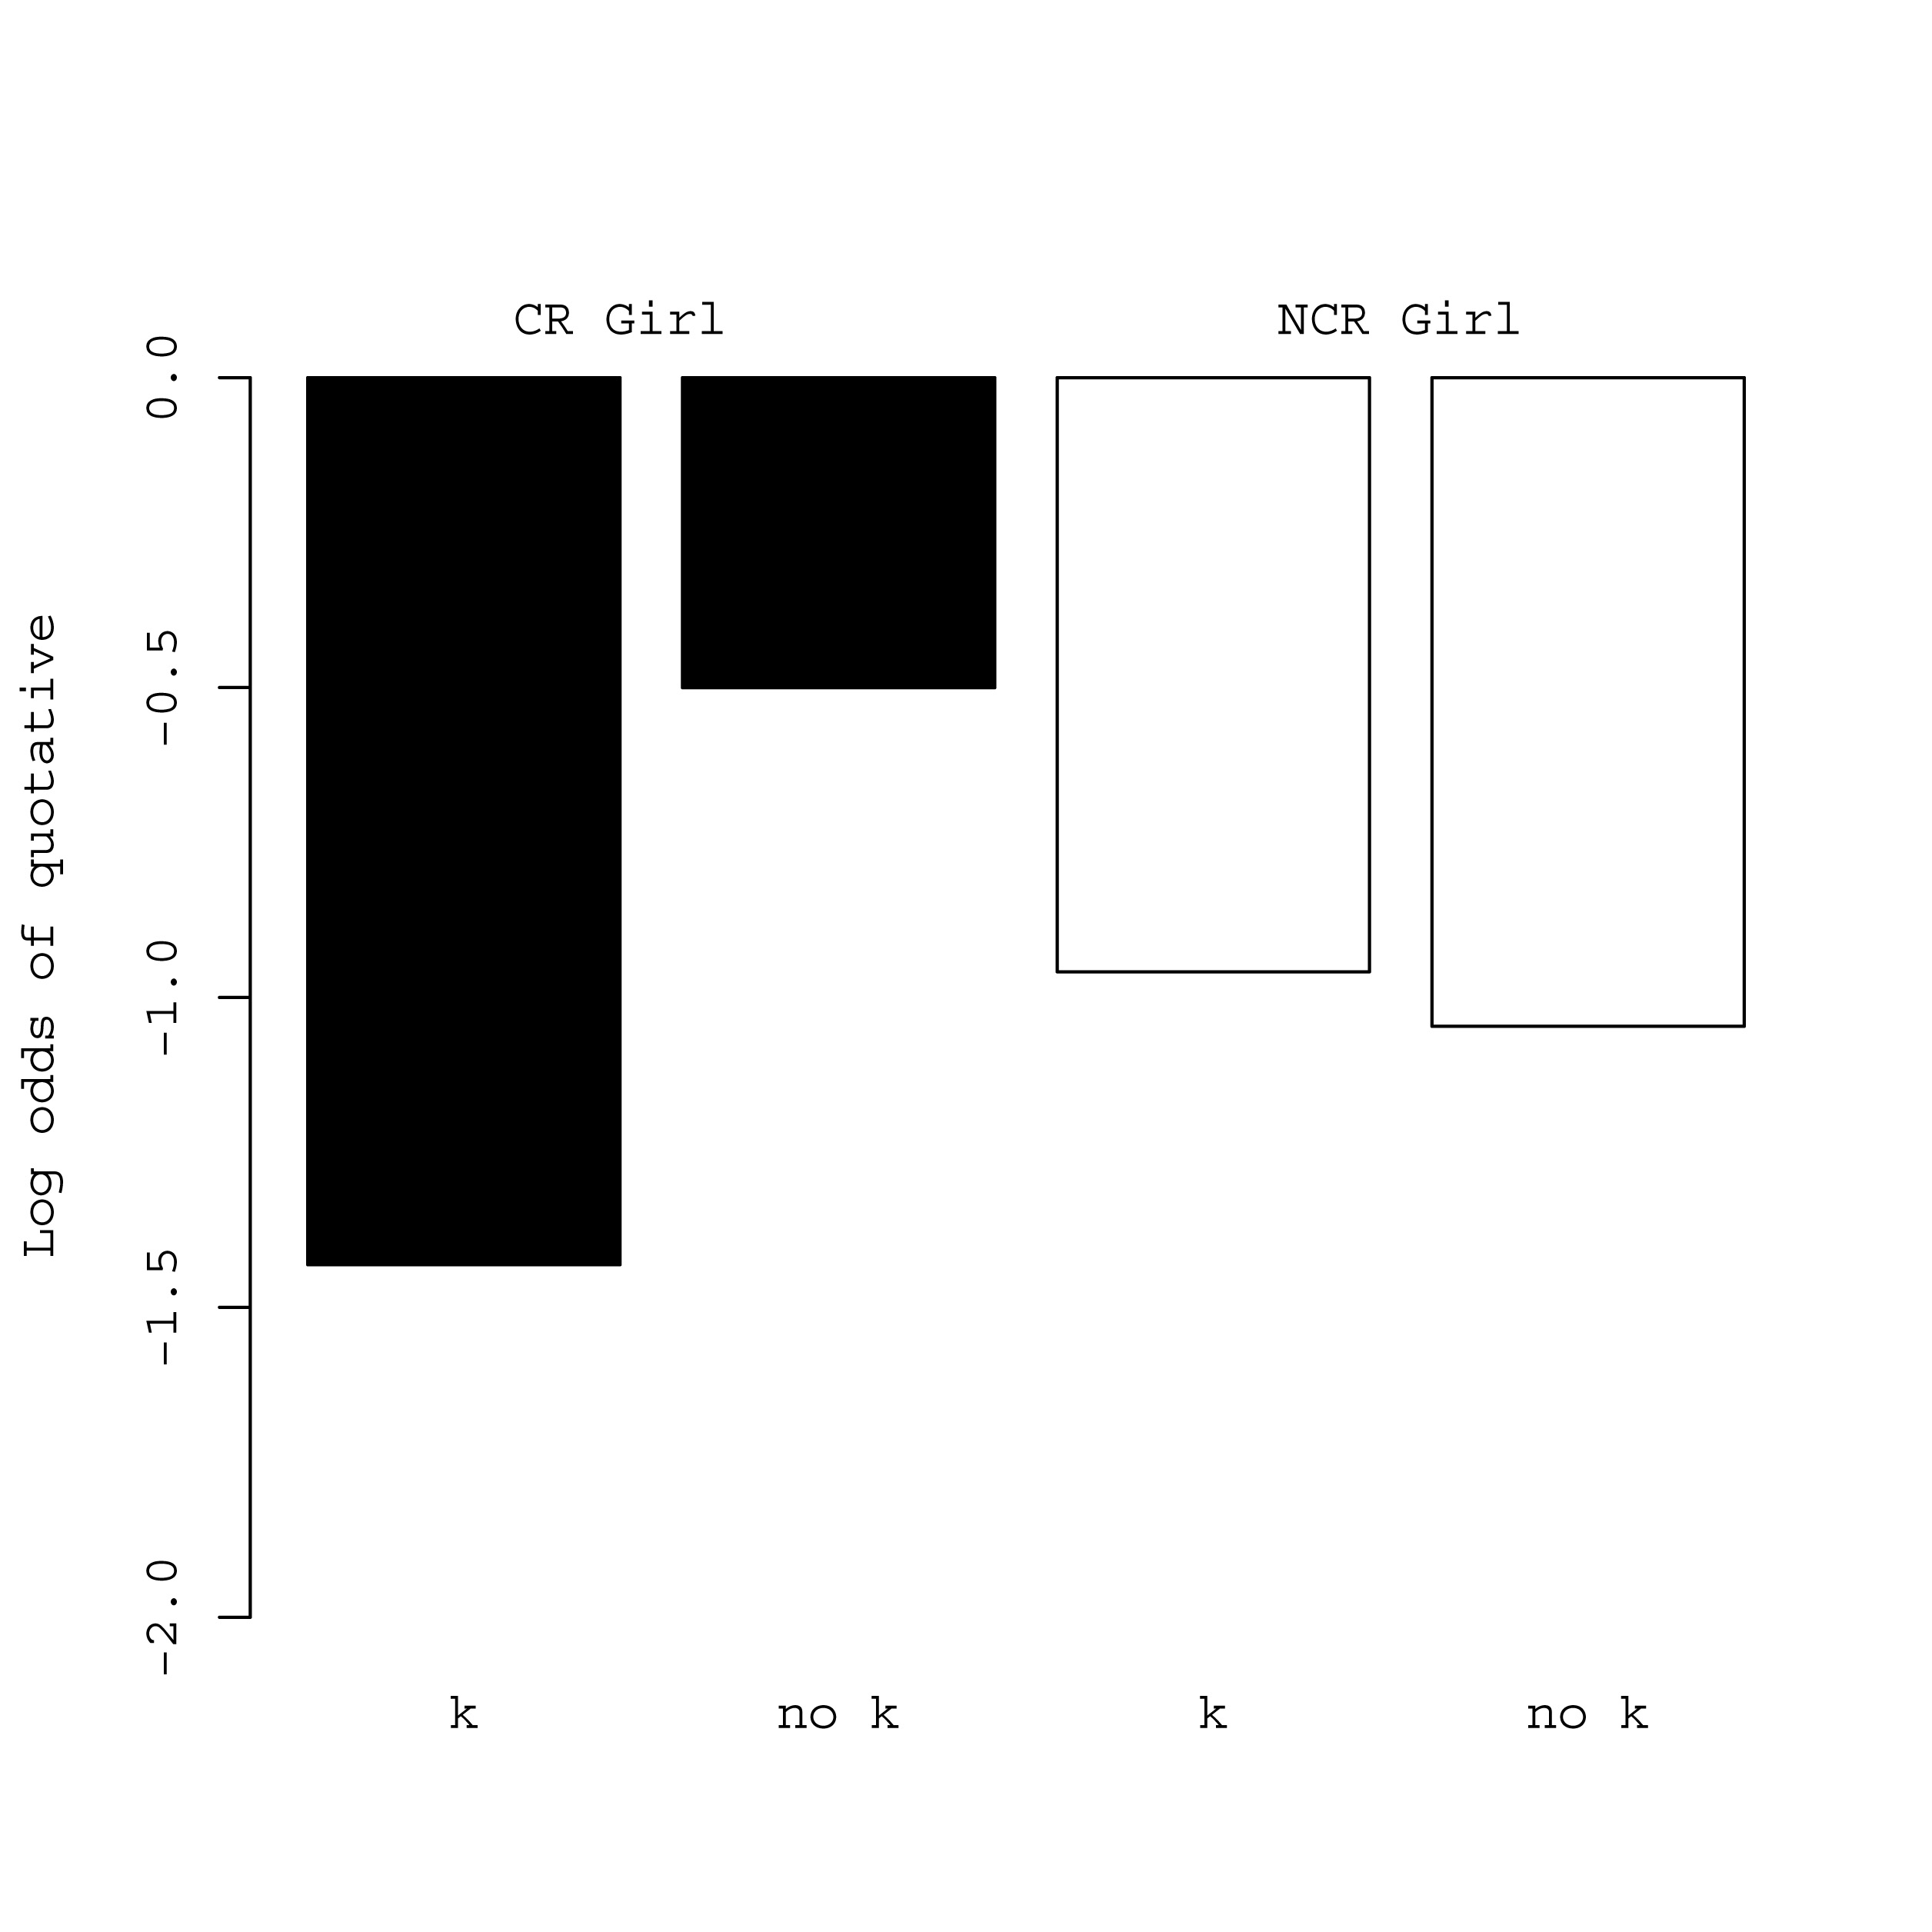
\includegraphics[height=5in]{images/kCR.jpg}
	\caption{Graph of the interaction between whether the /k/ was realised and whether the speaker was in a group who ate lunch in the CR (black) or not (white).  The graph is based on the model's predictions.  A higher value (i.e. closer to zero) on the y-axis indicates a greater likelihood that the token was quotative \textit{like}.}
	\label{fig:kCR-qdp}
\end{figure}



%no luck with eps, why???
%\begin{figure}
%\epsfxsize0.9\textwidth
%\epsffile{images/kCR.ps}
%\caption{Graph of interaction based on model's predictions of likelihood of quotative \textit{like} depending on whether the /k/ is realised and whether the speaker is in a group who eats lunch in the Common Room (CR, blue) or not (NCR, red)}. \label{prodinteract}
%\end{figure} 
%\epsfbox{kCR.eps}  this doesn't work either...


This interaction was not carried exclusively by quotative \textit{like}; the opposite trend of /k/ realisation was found for the discourse particle.  While CR girls were more likely to produce the /k/ in discourse particle \textit{like}, NCR girls were more likely to drop the /k/.

This interaction is not an artefact of the frequency of use of either the quotative or the discourse particle. Though they do not reach significance in the model, if frequency measures are included, the interaction between /k/ realisation and a girl's eating place is still significant.  This provides statistical evidence that the interaction is independent of the speaker-specific probability of producing quotative \textit{like}.  Interestingly, CR girls were significantly more likely to use the discourse particle than NCR girls (Wilcoxon, p$=$0.01).\footnote{This is based on the calculation presented in Section \ref{section:dplike}.}  But there is no interaction between the frequency of use of the discourse particle and whether the /k/ is realised.\footnote{This was tested with the percentage of all words that were the discourse particle, the percentage of all tokens of \textit{like} that were the discourse particle, and the ratio of quotative to discourse particle tokens produced by a speaker.}  Irrespective of how often a girl used quotative and discourse particle \textit{like}, she was more likely to realise the /k/ in quotative \textit{like} than in discourse particle \textit{like} if she was a NCR girl and more likely to drop the /k/ in the quotative than in the discourse particle if she was a CR girl.  For example, Juliet (PCs), Barbara (Relaxed Group), and Clementine (Trendy Alternatives) were all CR girls who were not particularly frequent users of quotative \textit{like} and they produced the /k/ more frequently in quotative \textit{like} than did some of their friends who used quotative \textit{like} more often.  However, these girls were more likely to produce the /k/ in the discourse particle than in the quotative, thereby patterning more similarly to their CR friends than with NCR girls who were also infrequent users of quotative \textit{like}.  

%I first observed this trend in the speech of Onya, who is a central member of the most rebellious group, The Real Teenagers.  In order to find out whether other NCR girls also followed this trend, Onya's speech was not included in the model.

%\subsection{Quality of \textipa{/ai/}}


In regard to monophthongisation, mean pitch, /l/ to vowel duration ratio, and following environment, both discourse particle \textit{like} and grammatical functions of \textit{like} behaved similarly when compared to quotative \textit{like}.  However, they involved different interactions: one with /k/ realisation and the speaker-specific probability of a token, and the other with /k/ realisation and the social grouping of the speaker.  Whereas the realisation of /k/ was linked to frequency of use for quotative \textit{like}, it did not appear to be linked to frequency of use for the discourse particle.  Phonetic differences between grammatical functions of \textit{like} and the discourse particle will be presented in the following section.

%The realisation of /k/ in quotative \textit{like} may be linked both to cognitive processes due to frequency effects and the manipulation of phonetic variables for the construction of identity.  However, socially-conditioned variation seems to be the only effect for /k/ realisation in the discourse particle.




\subsubsection{Model 3: Grammatical and discourse particle \textit{like}}


A mixed effects model was fit to the data comparing the discourse particle with grammatical functions of \textit{like}, modelling whether a token was one of the traditionally grammatical functions.  Speaker was included as a random effect.  Coefficients of the model's fixed effects are shown in Table \ref{dpgramcoeff} and the model's control variables are shown in Table \ref{dpgramcoeff-control}.  


% latex table generated in R 2.6.1 by xtable 1.5-2 package
% Mon Aug 11 13:13:39 2008
\begin{table}[ht]
\begin{center}
\begin{tabular}{lrrrr}
  \hline
 & Estimate & Std. Error & z value & Pr($>$$|$z$|$) \\
  \hline
(Intercept)    &  4.8433  &  1.8126 &  2.67&  0.0075\\ 
NUC F2       &  -0.4876 &  0.1546 & -3.15& 0.0016 \\ 
LV DURATION       &  -0.2231 &  0.6144 & -0.36& 0.7165 \\
GROUP=NCR                 &-0.4758   &  0.4666 & -1.02& 0.3079 \\ 
LV DURATION:GROUP=NCR     &  1.7159  &  0.8670 &  1.98& 0.0478 \\  
   \hline
\end{tabular}
\caption{Coefficients of fixed effects for Model 3, comparing the discourse particle with grammatical functions of \textit{like}.}
\label{dpgramcoeff}
\end{center}
\end{table}

% latex table generated in R 2.6.1 by xtable 1.5-2 package
% Mon Aug 11 13:13:39 2008
\begin{table}[ht]
\begin{center}
\begin{tabular}{lrrrr}
  \hline
 & Estimate & Std. Error & z value & Pr($>$$|$z$|$) \\
  \hline

preceded by pause  & -1.7516  & 0.3915 & -4.475 & $<$0.0001 \\
preceded by fricative 	& -0.9553   &  0.2503 & -3.82 & 0.0001 \\
followed by pause     &  -0.8570   &  0.4843  & -1.77 & 0.0768 \\
followed by V    &  0.7412 &    0.3799 &  1.95 & 0.0510 \\
followed by sibilant   & 1.4890  &   0.5040   & 2.95   & 0.0031 \\
followed by nasal    & 1.2666  &   0.5062   & 2.50 & 0.0123 \\
followed by other voiceless & 0.8749   &  0.4058 &  2.16 & 0.0311 \\
followed by other voiced  & 1.3631     & 0.3854   & 3.54 & 0.0004 \\  

   \hline
\end{tabular}
\caption{Coefficients of control variables for Model 3, comparing the discourse particle with grammatical functions of \textit{like}.}
\label{dpgramcoeff-control}
\end{center}
\end{table}


\noindent The preceding and following environment and the F2 value of a token's nucleus target significantly predicted whether a token was a grammatical function.  A token that was preceded by a pause or a fricative was less likely to be a grammatical function of \textit{like} than the discourse particle when compared with a token preceded by some other segment (p$<$0.0001).  The difference between tokens preceded by a pause as opposed to a fricative was approaching significance (p$=$0.06), with tokens preceded by a fricative being more likely to be a grammatical function.  

Tokens that were followed by an approximant were significantly less likely to be a grammatical function of \textit{like} than tokens that were followed by a sibilant (p$<$0.001), a nasal (p$<$0.05), a voiceless consonant of a different manner of articulation (p$<$0.05), and a voiced consonant of a different manner of articulation (p$<$0.001).  

Tokens with a higher F2 at the target of the nucleus (i.e. tokens with a nucleus that was less back) were less likely to be a grammatical function of \textit{like} (p$<$0.01).  This suggests that grammatical functions of \textit{like} were more likely to be produced with a backer diphthong nucleus than the discourse particle.  Between the two discursive functions, there was no significant difference in F2.

Also reaching significance in the model is an interaction between the /l/ to vowel duration ratio and whether or not the speaker ate lunch in the Common Room (p$<$0.05); tokens with a long /l/ relative to the vowel were more likely to be the discourse particle if produced by a common room girl and were more likely to be one of the grammatical functions if produced by a non-common room girl.  Together with the interaction from model 2, the results suggest that a word's phonetic realisation can depend on a combination of the word's grammatical function and the social characteristics of the speaker who produced it.

%  In NZE, the PRICE diphthong is un with a backer nucleus are considered more innovative \cite{onzebook}.  This provides evidence that grammatical \textit{like} was more likely to be produced with a more innovative realisation than the discourse particle.  

A summary of results from all three models is presented in Table \ref{tab:sumprodresults}.

  
\begin{table}[ht]
\begin{center}
\begin{tabular}{lr}
  \hline
 type & summary of traits \\
 \hline
 
 grammatical & low pitch   \\
             & more diphthongal \\
             & long /l/ to vowel duration ratio \\
             & shorter /l/ to vowel duration ratio for CR girls \\
             
             \hline
 quotative   & high pitch \\
             & less diphthongal \\
             & short /l/ to vowel duration ratio \\
             & more /k/ reduction for CR girls than NCR girls \\
             \hline
             
 discourse particle & low pitch \\
        		 & large F2 value but still diphthongal \\
             & long /l/ to vowel duration ratio \\
             & shorter /l/ to vowel duration ratio for NCR girls \\
             & more /k/ reduction for NCR girls than CR girls \\
  \hline

\end{tabular}
\caption{Summary of results from the first three statistical models.}
\label{tab:sumprodresults}
\end{center}
\end{table}


\section{Discussion}\label{sec:proddisc}

The results provide evidence that different functions of \textit{like} have different realisations.\footnote{It is possible that some of the variation observed between functions is due to effects of prosody and other phonetic cues not investigated here.  This is discussed briefly in Section \ref{sec:prosody}.}  The ultimate realisation depends on a combination of a token's grammatical function and the social grouping of the girl who produced it.  That the girls' realisations of \textit{like} were systematically different depending on the function of a token suggests that these items are stored in the mind in a way that maintains the distinction.  This is discussed in Chapter \ref{ch:disc} where I also describe implications of results from the perception experiments presented in Chapter \ref{ch:perc}.  The current section discusses how the results add to previous work on sound change, the discursive status of certain lexical items, and the link between phonetic reduction and a token's probability given the context.  
% 


\subsection{Frequency effects}

Previous studies provide evidence that token frequencies correlate with at least some phonetic variables.  The majority of previous studies have focused on vowel duration \cite{bybee2001,jurafskyetal2002,gahl-thyme}, but vowel quality and monophthongisation have also been shown to correlate with frequency measures \cite{munson2007,oprah1999}.  In these studies, monophthongisation, shorter vowel durations, and a more compact vowel space are associated with tokens that have a higher frequency.  In the SGH data, the different measures of relative frequency of use described in Section \ref{section:uselike} did not interact with monophthongisation, vowel duration, or the /l/-vowel duration ratio.  Given the amount of previous work that has found a relationship between token frequency and duration, it is surprising that no such effects were observed here.  This may be a result of using measurements that reflect the speaker-specific probability of producing a token in a given context (e.g., when speaking, or when producing a quotative) as opposed to an overall approximation of token frequency.  Alternatively, it may be related to the fact that, across all speakers, all of the analysed functions of \textit{like} would be classified as highly frequent in previous studies.  For example, \citeasnoun{bybee2002-lvc} treats words that are observed in corpus data equal to or more than 35 times per million words as high-frequency; all of the analysed functions of \textit{like} were more frequent than this for all speakers in the SGH data.  

In the model comparing the quotative with the grammatical functions, there is an interaction between /k/ realisation and the percentage of all quotatives that were quotative \textit{like}.  This interaction suggests that the speaker-specific probability of an item in a given context is linked to phonetic reduction in that item.  To demonstrate that this effect is independent of the effect of a girl's status as a CR girl or a NCR girl, I have fit a fourth mixed effects model with speaker as a random effect, modeling /k/ realisation and only including tokens of quotative \textit{like}. The model's output is shown for the test items in Table \ref{model4coeff} and for the control variables in Table \ref{model4coeff-control}.

   \begin{table}[ht]
\begin{center}
\begin{tabular}{lrrrr}
  \hline
 & Estimate & Std. Error & z value & Pr($>$$|$z$|$)  \\
  \hline
  
(Intercept)    &  -8.58498  &  3.75172  & -2.288  & 0.02212 \\
DIPH           &  0.92959  &  0.21775  & 4.269 & $<$0.0001 \\  
LV DURATION &  2.26894  &  0.84877  & 2.673  & 0.00751 \\
NUC F2   & 0.77772   & 0.28334  &  2.745 & 0.00605 \\
GROUP=NCR           &  1.47449  &  0.51989  & 2.836 & 0.00457  \\
PROB QUOTE          &  -0.04481  &  0.02160 & -2.075  & 0.03801  \\

   \hline
\end{tabular}
\caption{Coefficients of fixed effects for Model 4, modeling /k/ reduction for tokens of quotative \textit{like}.}
\label{model4coeff}
\end{center}
\end{table}

   
         


\begin{table}[ht]
\begin{center}
\begin{tabular}{lrrrr}
  \hline
 & Estimate & Std. Error & z value & Pr($>$$|$z$|$)  \\
  \hline
preceded by pause    &  -2.7829 &   1.78  & -1.57  & 0.1174 \\
preceded by fricative 	& 0.1268  &  0.38 &  0.34 & 0.7360 \\
followed by pause  &  1.1055  &  0.56  & 1.96 & 0.0495 \\
followed by V   &   1.1439 &   0.54 &  2.12 & 0.0341 \\
followed by sibilant & 2.2012  &  1.07 &  2.07 & 0.0389 \\
followed by nasal &  1.1754  &  0.74  & 1.59 & 0.1112 \\
followed by other voiceless & 0.4163 &   0.83 &  0.50 & 0.6156 \\
followed by other voiced  &  17.3702 & 989.60 &  0.02 & 0.9860 \\ 
   \hline
\end{tabular}
\caption{Coefficients of control variables for Model 4, modeling /k/ reduction for tokens of quotative \textit{like}.}
\label{model4coeff-control}
\end{center}
\end{table}

The model shows that there is a significant relationship between /k/ realisation and a token's Euclidean distance (p$<$0.0001) and /k/ realisation and the /l/ to vowel duration ratio of a token (p$<$0.05).  More diphthongal tokens and tokens with a longer /l/ relative to the vowel were more likely to have the /k/ present.  This is not surprising if monophthongisation, /l/ duration reduction, and /k/ dropping are all reductive processes.  Tokens that have the /k/ realised were also more likely to have a higher F2 at the nucleus target (p$<$0.01).

The key finding in this mo\-del was that for quotative \textit{like} both the spea\-ker's social grouping and how often she used quotative \textit{like} were linked to /k/ realisation.  NCR girls were more likely to realise the /k/ than CR girls (p$<$0.05) and the more a girl used quotative \textit{like}, the less likely she was to realise the /k/ in it (p$<$0.05).  Both social and frequency effects played a role in predicting whether the /k/ was realised.\footnote{Models fit only to the grammatical tokens and to the discourse particle tokens revealed that the social grouping and speaker-specific frequency did not play a significant role in whether or not the /k/ was realised (p$>$0.1 for the effects in both models).}

%, whereas in model 2, speaker frequencies of quotative and discourse particle \textit{like} do not appear to play a role in predicting /k/ realisation.  The interaction between social group and /k/ realisation is not an artefact of frequency.  Though there are more documented tokens of the discourse particle in the speech of CR girls than NCR girls, frequency of the discourse particle does not reach significance when tested in an interaction in the model. Additionally, given the previous work on reductive processes and frequency of use, we might expect that the CR girls would be less likely to realise the /k/ in discourse particle \textit{like} than the NCR girls because, as disccused in Section \ref{tab:diffquotes}, they appear to use the discourse particle more often.  But, if anything, the opposite was observed.  

%Using a larger corpus to test the influence of speaker-specific token frequency on sound change and phonetic variation is an interesting avenue for future research. 


Previous work has observed a relationship between the phonetic realisation of a word and its predictability based on contextual information \cite{jurafskyetal2002}: words that are more predictable given the preceding context undergo more reductive processes.  These findings help to interpret the results regarding the relationship between /k/-dropping and the percentage of a speaker's quotatives that were quotative \textit{like}.  If the contextual information indicates that a speaker is likely to produce a quotative, the probability of that quotative being \textit{like} (as opposed to some other quotative) is speaker-dependent.  Thus, for speakers who have a high percentage of quotatives that are \textit{like}, \textit{like} is more predictable in its local context; for these speakers, /k/ is more likely to be dropped.  Conversely, for speakers who have a lower percentage of quotatives that are \textit{like}, \textit{like} is less predictable in its local context and the /k/ is less likely to be dropped.

This supports previous findings that words that are more predictable given the preceding context undergo more reduction.  Further, it indicates that predictability needs to be considered at the level of the individual speaker; not all words are equally predictable in all contexts for all speakers.

%If phonetic reduction is more likely to be observed when a word is more likely to occur in a given context, the same cognitive mechanisms would predict that phonetic reduction in an item is more likely to occur if, in a particular context, the likelihood of a speaker producing that item is high.  If the contextual information indicates that a speaker is likely to produce a quotative, the probability of producing \textit{like} is speaker-dependent.  The results indicate that when this speaker-specific probability is high, /k/ is more likely to be dropped.  This provides evidence that, in addition to contextual predictability affecting phonetic realisations, the probability of a particular speaker producing a word in a context also affects phonetic realisations.

It is possible that phonetic patterns that derive from speaker-specific, context-dependent probabilities could be exploited as a stylistic resource.  Such re-appropriation of phonetic variables could have led to the differences in /k/ realisation observed between CR and NCR girls.  Stylistic resources are constantly recombined in a process of bricolage \cite{hebdige1984,eckert2008}.  While work such as that by \citeasnoun{milroymilroy1978} has focused on a community or social group's adoption of (and reassignment of meaning to) variables used by another group, it is also possible that phonetic variability originally driven by speaker-specific probabilities could be manipulated for stylistic means.  Due to the multidimensional nature of the stylistic components, the model presented in Chapter \ref{ch:disc} predicts that socially-conditioned phonetic variability could arise from probabilistic distributions of the variables based on non-social factors.




%This would be consistent with the predictions of an exemplar model, which will be discussed in Chapter \ref{ch:disc}.  

%Another interpretation is that /k/ dropping is linked to identity construction; girls who choose to use quotatives other than quotative \textit{like} may also choose to realise the /k/ in quotative \textit{like} when they produce it in order to diverge from the more frequently used pronunciation.  This would be consistent with results from Model 1, but the social make-up of the girls who would choose to do so is less clear. [needs more] 

%The /k/ in quotative \textit{like} should be dropped for individuals who use a higher percentage of quotative \textit{like} compared to non-quotative functions of \textit{like}.  

%[This suggests that the relationship between /k/ realisation and percentage of quotatives that were \textit{like} could be due to (a) social construction of identity through /k/ realisation or (b) predictability of producing quotative \textit{like} given the likelihood of that particular speaker producing a different quotative.  Both interpretations involve social motivation, either directly on the realisation of the phonetic variable or indirectly through the choice in which quotative to use.  ]this needs to be thought through more.

%...These two possible interpretations are not necessarily mutually exclusive; speakers express their identities through choosing which quotative to use and may realise the /k/ 




\subsection{Special status of discursive tokens}\label{sec:statusofdisc}

The only socially-conditioned phonetic variation in the production of \textit{like} was found when observing two discursive functions, quotative \textit{like} and discourse particle \textit{like}: a token was more likely to be quotative \textit{like} if the /k/ was not realised and it was produced by a CR girl or if the /k/ was realised and it was produced by a NCR girl.\footnote{Of course, frequency of use was related to social characteristics.  Here, however, I am focusing on socially-conditioned phonetic variation that was not derivative of frequency.}  Why might this be?  I argue that their discursive nature and their frequent use make them probable targets of sociophonetic variation.

The frequent occurrence of these discursive items may ensure their status as loci of socially meaningful phonetic variation.  Work in sociophonetics has demonstrated that the realisations of frequent items can be socially meaningful and manipulated stylistically \cite{oprah1999}.  The frequent repetition of quotative and discourse particle \textit{like} would provide ample opportunity for these words to become layered with social meaning, but frequency alone can not explain why particular pronunciations become imbued with social meanings.  Because patterns of /k/ realisation in quotative and discourse particle \textit{like} were in the opposite direction, this result can not be a matter of ease of processing.  I believe that socially meaningful phonetic variation in discursive words is a result of the words themselves carrying socially indexical meanings.

%It is possible that the realisations slang terms and discursive uses of common words are prime targets for the manipulation of phonetic variables in the construction of one's identity.  The use of slang in general is closely related to identity construction (Bucholtz 2001).  Slang serves as a method of constructing an identity that separates adolescents from adults as well as children, and it also serves to construct distinct identities within youth culture.  ``Variation in slang use, like music fandom, clothing, and hairstyles, allows teenagers to identify themselves with some of their peers while differentiating themselves from others; in short, it enables teenagers to produce distinctive linguistic and cultural styles'' (Bucholtz 2006: 251).  Likewise, vernacular forms of words that are not considered slang, such as quotative and discourse particle \textit{like}, can also index social information, whether it be youth or membership to a particular social group.

Discursive items, which I define as words used in informal speech situations that are not considered traditionally grammatical but are used across generations of speakers, come to be indexed with social meaning through variation and eventual associations with particular social groups.  In her discussion of slang, Bucholtz explains how

\begin{quote}
	variation in slang use, like music fandom, clothing, and hairstyles, allows teenagers to identify themselves with some of their peers while differentiating themselves from others; in short, it enables teenagers to produce distinctive linguistic and cultural styles. \cite[251]{bucholtz2006}
\end{quote}

\noindent  Both quotative \textit{like} and discourse particle \textit{like} can be used similarly, a point I will return to shortly.

Lexical items with particularly socially-indexical meanings can serve as vehicles for phonetic variables that in themselves index social meaning.  \citeasnoun{eckert1996} found that words like \textit{all-nighter} and \textit{fight} could be realised by Burnouts with an especially raised \textipa{/ai/} diphthong.  The extreme phonetic realisation, which was associated with the city, emphasised the toughness and rebelliousness that the lexical items themselves also indexed.  \citeasnoun{chun2007} found that the pronunciation of the phrase \textit{oh my god} was stylistically manipulated and she argued that words and phrases can index social characteristics, especially when used in conjunction with socially meaningful phonetic variants.  That discursive lexical items in particular often index `youth', `coolness', and stances associated with a particular social group suggests that their phonetic realisations will be readily manipulated as a means of emphasising social characteristics such as these.




%Work on grammaticalisation has shown a correlation between lexical frequency and whether a word has undergone an innovation in meaning.   Find: Traugott, E.C. 1989. On the rise of epistemic meanings in English: An example of subjectification in semantic change.  Language 65, 31-55.  And w



In terms of \textit{like}, there are two levels of association in language ideology: youth culture as distinct from non-youth culture and between the different groups within youth culture.  Both quotative and discourse particle \textit{like} are discursive items associated in language ideology with youth culture in the US and the UK \cite{daileyocain2000,buchstaller2006}, making them prime potential candidates in which to observe phonetic variation that signals `youth' as well as characteristics associated with youth culture.  Though comparable work has yet to be carried out in New Zealand, conversations between girls at the school suggest that speakers of New Zealand English associate \textit{like} with youth culture.  After taking part in the perception experiments discussed in Chapter \ref{ch:perc}, several girls wanted to share their opinions on the discursive functions of \textit{like}, both with me and with each other.  In the conversation between Theresa and Esther (Christians) shown in Example \ref{momdoesnotlikelike}, Theresa explained how her mother did not understand why she used \textit{like}.  Esther's response suggested that the available alternative was undesirable.



\sent{

Theresa and Esther, Christians. Interview, 24-10.

\vspace{3 mm}
	
 Theresa: no but they're so bad with like \newline
          \hspace{10 mm} Mum Mum's like why do you say that \newline
          and um
 
 Esther:  `cause otherwise we'd have to use the word said \newline
 					and that would just be annoying
 					
}\label{momdoesnotlikelike}
%(Interview 1:43-2:02)
\vspace{5 mm}


\noindent Though girls in every group at the school used them, discursive functions of \textit{like} were particularly associated with the PCs.  In Example \ref{PCsuselike}, Ricky and Marissa talked about how Joanna and Alissa, two PCs, were frequent users of the discursive functions of \textit{like}.

\sent{

Ricky and Marissa (Goths). Interview, 14-10.

\vspace{3 mm}

Ricky: in assembly one time when Joanna and Alissa were talking \newline   

Marissa: and we sat there \newline
we're like	one . 

Ricky:  duh duh duh duh duh duh duh duh [counting on fingers]

Marissa: duh duh  [counting on fingers]\newline
I ran out of fingers within the first five seconds 

[laughter]

Marissa:  she r- she ran I ran out of fingers \newline
   within the first five seconds

Ricky:  `cause she uses it more than I than most people 

 
}\label{PCsuselike}
%(Interview 2:45-3:07)
\vspace{5 mm}


\noindent Interestingly, the PCs whose speech was analysed were not the highest users of quotative \textit{like}.  Even Emma, one of the girls explicitly mentioned by others as someone who was a frequent user of \textit{like}, was not one of the most frequent users of either quotative or discourse particle \textit{like} based on the measures presented in Section \ref{prod-like}.  The perception that she was a frequent user likely came from her frequent use of the discourse marker and approximant adverb combined with her highly visible status at the school.  

Despite \textit{like} being associated with the PCs, girls in other groups were highly aware that they used it as well.  Before the segment shown in (17), Marissa suggested that they try to avoid saying \textit{like} during the morning break.  Ricky, knowing how frequently and automatically they used it, stated simply that ``it won't work''.  The widespread use of the lexical items combined with their association with a particular group served to make the discursive functions of \textit{like} a target of socially-meaningful phonetic variation within the school.
%(Interview 2:34)

%An alternative interpretation is that quotative and discourse particle \textit{like} arecan occur with an identical preceding context, and to avoid ambiguity, speakers may maintain a phonetic contrast between the items.  Different speakers or groups of speakers could contrast them similarly to each other (as with monophthongisation) or differently (as with /k/ realisation).  Results show that not more of an effect for ambiguous contexts.




Another word with a discursive use that seemed to have a distinct pronunciation at the school from the traditionally grammatical function was the word \textit{yes}.\footnote{I have also noticed this difference among New Zealanders outside of SGH.}  When girls used \textit{yes} as an exclamation, the vowel was backed and centralised, which strongly contrasted with the fronted, raised variant used in the agreement form of \textit{yes} and most other words containing this vowel.  The girls were highly aware of this distinctive pronounciation of exclamation \textit{yes} and in writing they spelled it as `yuss'.  This is another example of how words with discursive meanings can be used in conjunction with distinct pronunciations.


\subsection{Changes in progress}
In NZE, the diphthong \textipa{/ai/} is involved in two on-going sound changes: the nucleus is shifting back, a phenomenon known as diphthong shift, \cite[149]{onzebook} and the diphthong itself is becoming more monophthongal, which is referred to as glide weakening \cite{onzebook,chartres2008}.  Realisations that are innovative in terms of both glide weakening and diphthong shift can be produced by the same individuals \cite{chartres2008}.  In the current study, the function of \textit{like} was predictable both by how diphthongal and by how backed the vowel was.  A backed nucleus was associated with grammatical functions, while a monophthongal vowel was found in the quotative.  This suggests that there is a conflict in terms of innovation: quotative \textit{like} was produced with the most innovative realisation in terms of glide weakening and the grammatical functions were produced with the most innovative realisation in terms of diphthong shift.  Results described in \citeasnoun{chartres2008} indicate that both glide weakening and diphthong shift are led by males in NZE.  Informal discussions with colleagues who are from New Zealand suggest that while a backed nucleus is highly associated with males, a monophthongal realisation is not. Thus, girls at the school may avoid producing variants associated with males and this may be particularly true in contexts such as discursive words that strongly index identity, especially with the discursive functions of \textit{like} that are highly associated with females.  Another possibility is that the discursive functions of \textit{like} are more likely to carry primary stress in a sentence.  Stressed tokens tend to be more peripheral in a speaker's vowel space than unstressed tokens.  However, there was no significant difference observed for vowel duration or whether the pitch was moving or stable, both of which are other acoustic cues for stress.  A study on the ideology surrounding the changes in progress in which \textipa{/ai/} is involved may help to shed light in interpreting the findings presented here.

\subsection{Prosody and phonetic variation}\label{sec:prosody}

It is well established that prosody can affect articulation.  Vowel duration \cite{edwardsbeckman1992}, formant transitions in diphthongs \cite{woutersmacon2002}, glottalistion \cite{dilleyetal1996}, and consonant realisation \cite{fougeronkeating1997} all appear to be linked to prosodic position; greater articulatory effort tends to be observed at prosodic-domain edges \cite{fougeronkeating1997}.  While only one of the analysed tokens in the current study occurred at a sentence boundary, this does not ensure that the observed phonetic differences between the different functions of \textit{like} were not in fact due to the token's prosodic position in the sentence.  When compared to the discourse particle, quotative \textit{like} was more likely to have a shorter /l/ to vowel duration ratio and a more monophthongal vowel; both of these might be expected if the quotative was more likely to occur in a prosodically less prominent position.  However, we might also expect to observe both a shorter vowel duration and a lower rate of /k/ realisation in the quotative.  In actuality, there was no significant difference in vowel duration, and /k/ realisation depended on social characteristics of the speaker.  While some of the phonetic differences observed between the different functions may be related to frequency, it is unlikely that all of them, /k/ realisation in particular, resulted from prosodic differences.  Further work in this area is beyond the scope of this book, but it would certainly be a worthwhile avenue for future work, especially given the fact that the majority of work investigating the effects of prosody on articulation is done in the laboratory.\footnote{One notable exception to this is Cole, Kim, Choi and Hasegawa-Johnson (2007), who used speech from a corpus of radio news.\nocite{coleetal2007}}  

\subsection{Identity Construction}\label{sec:idconstruction}

 

What is the meaning behind the stylistic variation of /k/ realisation?\footnote{Whether or not the realisation of /k/ is a variable undergoing a sound change in progress is not relevant for this discussion.  Either way, it is being used stylistically in the construction of the girls' social identities.}  Speakers actively manipulate linguistic variables and non-linguistic qualities to construct their identities.  The variation of /k/ in quotative and discourse particle \textit{like} is no exception.  Zwicky (1997) outlines two internal psychosocial mechanisms for the acquisition of identity: identification and avoidance.  He argues that an individual can model their behaviour based on characteristics of those who they believe they are similar to or who they would like to be similar to (Identification).  Conversely, individuals can reject behaviour of people who they wish to dissociate themselves from or who they do not believe themselves to be similar to (Avoidance).

At Selwyn Girls' High, norms of dress and behaviour were set by the CR girls.  These girls did not adopt `normal' qualities so much as they determined which linguistic and non-linguistic factors were considered to be `normal' at the school.  In the results presented in this chapter, the CR girls consistently displayed a strong tendency to drop the /k/ in quotative \textit{like} and to produce the /k/ in discourse particle \textit{like}.  They conformed to each other in an act of identification.  It is also possible that adopting these trends was an act of avoidance of realisations produced by particular individuals from a NCR group.

It is unlikely that NCR girls were conforming to each other's speech.  There was no evidence of identification in terms of clothes, values, or life\-styles across the different NCR groups; there was not a common so\-cially-con\-structed identity that united them.  In the production of \textit{like}, NCR girls displayed the opposite trend as CR girls: they were more likely to produce the /k/ in quotative \textit{like} than in discourse particle \textit{like}.  The trend was less robust than the trend observed in the speech of the CR girls.  It is clear, however, that NCR girls did not adopt the variation observed in the speech of the CR girls.  In fact, they showed the opposite trend, providing evidence of avoidance.  They rejected the norms of the CR girls and their trends in production were contrary to those of the CR girls from whom they wished to distance themselves.  

The PCs were an especially salient group.  They were talked about by other groups and were always named first when identifying groups at the school.  The discursive functions of \textit{like} were particularly associated with them in the school's language ideology.  Taken together, this suggests that it is possible that NCR girls were diverging from the PCs or particular individuals in the PCs rather than from the CR girls as a whole.  While CR girls in groups other than the PCs may have been accommodating to the PCs, the evidence does not necessarily support this.  The PCs whose speech was analysed for this study did not display the strongest trends in the CR direction.  This is true even for those girls who were core members of the PCs, such as Emma and Tracy.  It is likely that CR girls as a whole converged on each other's speech rather than accommodated to that of a single group.

That the trends of /k/ realisation result from identification and avoidance finds support in the NCR girls' rejection of non-linguistic norms.  There is a close relationship between linguistic features used by a speaker and that speaker's choice in other stylistic components, such as clothing \cite[89]{bourdieu1991}. Choice of clothing was fairly consistent across the different CR groups, while many NCR girls chose to wear clothes that were dissimilar to those worn by the CR girls.  The NCR groups' divergence in choice of clothing took a variety of forms and it is likely that they also deviated from the CR norms in terms of phonetic variables that have not yet been investigated.  In terms of /k/ realization for quotative and discourse particle \textit{like}, the different NCR groups seem to have diverged from CR girls in a similar direction.  Of course, there was still a great deal of variation across the different NCR groups, even in terms of /k/ realisation.  Trends in the speech of individual girls will be discussed in the next section.

The observed differences between CR and NCR girls are a result of identification and avoidance.  CR girls' similarities in production of \textit{like} are a result of identification with one another and conforming to each other's speech (and possibly avoiding speech patterns of the NCR girls) and NCR girls' similarities may be due to avoidance and a rejection of the CR girls' norms.




\subsubsection{Variation at the individual level}\label{theindividual}

In this section, I discuss the patterns of /k/ realisation exhibited by different individuals.  I argue that a strong NCR trend in production (i.e. they were more likely to drop the /k/ in discourse particle \textit{like} than in quotative \textit{like}) is associated with individuals who were likely to reject norms, and that a strong CR trend in production (i.e. they were more likely to drop the /k/ in quotative \textit{like} than discourse particle \textit{like}) is associated with a wider range of people: those who actively embraced norms as well as others with alternative motivation.  The order of individuals (from speaker with the strongest NCR trend to speaker with the strongest CR trend) is shown in Table \ref{tab:indiv}.  The coefficients are based on a separate production model fit to the data, modelling the likelihood of producing the /k/.  Included in the model was an interaction between whether or not the token was quotative and the random effect of the speaker.  The following environment was included as a fixed effect.  The estimate for each speaker is the difference between random effect coefficients when the token was the discourse particle and when it was the quotative.  The coefficients in the table are a reflection of a speaker's likelihood of producing the /k/ in discourse particle \textit{like} relative to quotative \textit{like}.  A larger coefficient means that a speaker was more likely to produce the /k/ in the quotative than in the discourse particle; the more negative the coefficient, the more likely a speaker was to exhibit a strong CR trend in production.  These results are also presented in \citeasnoun{dragerhay2012}.



\begin{table}[htbp]
\begin{center}
\begin{tabular}{lrrrr}
  \hline
Speaker & Sub-group & Group & Estimate \\
\hline
Barbara	  &  Relaxed Group & CR   &  -1.84791\\
Clementine	& Trendy Alternatives  & CR  & -1.71651\\
Rochelle	&  Rochelle's Group & CR    &  -1.47306\\
Rose	    &  Relaxed Group  & CR  &  -1.33595\\
Holly	  &  Sonia's Group & NCR   &  -1.26401\\
Betty	  &  Sporty Group   & CR   &  -1.01303\\
Meredith  & Goths         & NCR  &	 -0.85033\\
Juliet	& PCs &       CR        & -0.74285\\
Tracy	  &  PCs            & CR   &  -0.72341\\
Bianca	&  Geeks         & NCR  & -0.67159\\
Emma	&  PCs             & CR     &  -0.65743\\
Tania	  &  Goths          & NCR &  -0.59702\\
Katrina	& Relaxed Group  & CR   &   -0.40379\\
Sarah	  &  Real Teenagers & NCR & -0.38485\\
Justine	&  Trendy Alternatives &       CR    &  -0.38075\\
Mariah	& Geeks &    NCR        &   -0.14698\\
Theresa	& Christians & NCR     & -0.09286\\
Christina	& Trendy Alternatives & CR &  0.015748\\
Jane	& BBs  &             CR    &  0.13346\\
Marissa	& Goths          & NCR  &  0.281689 \\
Kanani  & Sporty Group   & CR  &  0.561684\\
Marama	& Pasifika Group & NCR     & 0.589017\\
Patricia & Sporty Group  & CR  &	0.746599\\
Isabelle & Real Teenagers & NCR &	0.967743  \\
Vanessa	& Goths     & NCR     & 1.024424\\
Esther	& Christians     & NCR & 1.130588\\
Joy	    & Geeks     & NCR     & 1.789199\\
Santra	& Goths     & NCR    & 1.994998\\
   \hline
\end{tabular}
\caption{Likelihood of an individual producing /k/ in discourse particle \textit{like} compared to quotative \textit{like}.  Estimates are based on a separate model fit to the production data modelling the likelihood of /k/ realisation, with an interaction between the random effect of a speaker and whether the token was the quotative or the discourse particle.  The presented estimate for each speaker is the difference between random coefficients when the token is a discourse particle and when it is a quotative.}
\label{tab:indiv}
\end{center}
\end{table}


The girl who showed the strongest NCR trend (she was most likely to produce the /k/ in quotative \textit{like} and drop the /k/ in discourse particle \textit{like}) was Santra.  Santra was the central member of the Goths.  She was the only goth who wore all black; she was the goth who gave the Goths their name.  She questioned everything, loudly and boldly.  She had very strong political and social views and she was the only openly bisexual girl in Year 13.  If anyone at the school was the most likely to reject norms and rebel against conformity, it was Santra.\footnote{Another girl who was highly likely to reject norms was Onya (the Real Teenagers), whose speech was not analysed because she did not take part in the perception experiment.  However, it is worth noting that it was upon noticing the NCR trend in Onya's speech that led me to look at the variable in the speech of the other girls.}  Perhaps it is unsurprising that out of all of the girls whose speech I analysed, Santra's realisations of quotative and discourse particle \textit{like} were least similar to those of the CR girls.

Other NCR girls also exhibited strong NCR trends.  These include Va\-nessa (The Goths), Joy (The Geeks), Isa\-belle (The Real Teen\-agers), Ma\-rama (The Pasifika Group), and Esther (The Christians).  These were girls who expressed feeling different from other girls at the school and they were proud of these differences. 

The girl with the most atypical trend for a CR girl was Patricia from the Sporty Group.  Though the majority of her tokens of quotative \textit{like} had the /k/ dropped, she was less likely to produce the /k/ in discourse particle \textit{like} than in quotative \textit{like}.  Patricia had some M\=aori ancestry, though she did not identify strongly as M\=aori.  I mention this because her speech patterns in terms of \textit{like} were similar to those of two other non-P\=akeh\=a girls, Marama and Kanani, and because she had some features of M\=aori English in her speech despite not identifying strongly as M\=aori.  She was also not a central member of her group.  Though she liked the Sporty Girls, her closest friends went to schools other than SGH.  Most of her social time while away from school was with these other girls.  As shown in Example \ref{ex:patricia1}, Patricia felt disconnected from the majority of girls at SGH.


\sent{

Patricia, The Sporty Girls, 24-07

\vspace{3 mm}
 
 Patricia: oh yeah \newline
 I just come here and I learn pretty much 
 
 [laughter] 
 
 Patricia: yeah
 
 KD: that's good
 
 Patricia: yeah I get along with the people but \newline
 					 I don't really . know \newline
 						you know . that many people really well \newline
 						like . say hi to them and stuff but yeah
 
 KD: mm
 
 Patricia:	and it was kind of hard \newline
 					`cause I came in at the start of fourth form \newline
 						and everyone had made their groups \newline
 						. and known each other and stuff
 						
KD:	oh yeah
 
Patricia:	and I was just like \newline
 						yeah I had to try and fit in then
}\label{ex:patricia1}

\noindent In fact, Patricia felt so disconnected from The Sporty Girls that she did not refer to them as her group.  When using the term `my group', she was referring to her friends who went to other schools, as shown in Example \ref{ex:patricia2}.


\sent{
Patricia, The Sporty Girls, 24-07
\nopagebreak
\vspace{3 mm}

Patricia:		I reckon I'm a lot different at school than I am to the outside school actually

KD:  really?

Patricia: yeah

KD: how?

Patricia: um . `cause I'm more comfortable around you know my own friends and my own group
}\label{ex:patricia2}


\noindent It is likely that Patricia conformed to the patterns of her friends outside of SGH, with whom she identified more strongly, rather than to those of the SGH group with whom she was friendly.


 
%I have several recordings of Kanani imitating the speech of what is either a California valley girl (a character she would perform when imitating me) or a CR girl.  These tokens were not included in the analysis, but I would like to analyse them in the future to determine how accurately she imitates the speech of CR girls and myself.

That girls such as Santra, Marama, and Patricia did not embrace the norms established by the CR girls suggests that their pattern of /k/ realisation for quotative and discourse particle \textit{like} was an active manipulation of a linguistic variable to construct their identity as someone who was distinct from the CR girls.

Like Patricia, Kanani (Sporty Girls) was more likely to produce realisations of \textit{like} associated with NCR girls.  Kanani, who was of Pacific Island descent, used to be in the Pasifika Group but changed to the Sporty Girls at the beginning of the year.  As a result of the switch, the Pasifika Group was no longer friendly toward her and she wanted nothing to do with them.  Though she was extremely friendly and readily accepted by girls in her new group, she resisted becoming a part of the group entirely and would instead seek out my company, sometimes even when I was sitting with another CR group.  Outside of school, she spent time with her new group of friends, with friends from other schools, and with her family.  Given her previous membership in a NCR group and her continued dismissal of CR norms, it is not surprising that she did not entirely adopt the production patterns of the CR girls. (Though see more on Patricia and Kanani in Chapter \ref{ch:concl}.)
%(and perhaps also their use of quotatives other than \textit{like} and their tendency to realise the /k/ in quotative \textit{like}) 

Two of the Goths, Meredith and Tania, did not exhibit strong NCR trends and were instead more likely to produce /k/ in discourse particle \textit{like} than in quotative \textit{like}.  Tania was previously a member of a CR group (Relaxed Group) but had left the group because she felt that the friendship contributed to her eating disorder.  Though she was no longer friendly with girls in the Relaxed Group, she interacted occasionally with girls in other CR groups, especially toward the end of the year.  She did not reject their expectations as actively as many of her friends in the Goths and her realisations of \textit{like} more closely resembled those of the CR girls.  

That Meredith's realisations of \textit{like} patterned more similarly to the CR girls than the NCR girls is surprising; I expected them to pattern with those of her best friend, Vanessa.  The motivation behind her adoption of CR trends is rather speculative.  It's possible that she adopted variants produced by her other close friend, Tania.  It is also possible that she diverged from the speech patterns of Isabelle, with whom she had a falling out earlier in the year.  It is also possible that she was less opposed in general to the norms of the CR girls.  She wore clothing that could have been worn by members of the Relaxed Group and she had lost a great deal of weight in the previous year, perhaps signalling a willingness to conform to society's expectations of beauty.  She was also the Goth who, as discussed in Chapter \ref{ch:ethnography}, had first claimed to be ``normal''.  After being met by silence from her friends she changed her stance toward normalcy, claiming that she was weird and stating that normal was boring.  Interestingly, both Meredith and Tania were among the girls with the highest rates of discourse particle \textit{like}.  This function was used more often by, and associated with, CR girls.  Though they were in a NCR group, it seems that Meredith and Tania had patterns of \textit{like} that resembled those of CR girls.  That the patterns in their production of \textit{like} were not consistent with those observed for other girls in their group demonstrates how stylistic resources need not have a one-to-one relationship with a social group; there may be alternative motivation behind some variants observed.  

Another NCR girl who produced CR-like trends in her production of \textit{like} was Holly (Sonia's Group).  Both Holly and Sonia talked about the PCs as though they were friends, though I never saw them interact.  Holly did not eat lunch in the CR nor did she sit with the PCs, but from the way she talked about them, it was clear that she looked up to them. She may have adopted similar speech patterns in terms of \textit{like} as a result of identifying with the PCs.




\subsection{Reflection on influence from researcher}

Social characteristics of a researcher can influence the realisation of phonetic variables \cite{rickfordetal1994}.  Additionally, varying levels of familiarity with a researcher can influence production \cite{cukoravilabailey}.  How, then, can I be sure that my presence and the constantly shifting interpretation of my identity did not influence the girls' realisations of \textit{like}?  The truth is, I can not be sure and in fact, it is unlikely that my presence did not influence their production.

I grew up using both quotative and discourse particle \textit{like} and my native dialect (Southern California English) is a dialect closely associated with discursive functions of \textit{like} in language ideology in the U.S. It is possible that a similar stereotype exists in New Zealand.  In fact, different girls at the school informed me that they started using \textit{like} after watching the movie `Clueless', which was set in Southern California.  It is possible that some of the girls accommodated to, or diverged from, my pronunciations of \textit{like}.  For this reason, I present a short analysis of \textit{like} from my own speech, both when speaking to CR girls and when speaking to NCR girls.

\subsubsection{Methodology}
Tokens from my speech were selected from recorded interviews with girls whose speech was analysed for the production results presented in this chapter.  Because analysis of their speech displayed socially-conditioned variation only for quotative and discourse particle \textit{like}, these were the functions analysed for my speech.  Tokens from interviews with CR girls and NCR girls were analysed separately in order to determine whether we had converged on each other's speech.  10 tokens of quotative \textit{like} and 10 tokens of the discourse particle from interviews with girls from CR and NCR groups were analysed, resulting in a total of 40 tokens of \textit{like}.  Results based on the girls' speech indicated that the socially-meaningful phonetic variable was the realisation of the \textipa{/k/}.  Therefore, this was the only phonetic cue analysed for tokens from my speech.

\subsubsection{Results}
The analysis demonstrates that I overwhelmingly realised the \textipa{/k/}, regardless of the function of \textit{like} and regardless of who I was speaking to.  Of all 40 tokens analysed, only three did not have the \textipa{/k/} present.  Two of these were when speaking to NCR girls and included both a quotative and a discourse particle and the other token was a quotative when speaking with girls in a CR group.  

\subsubsection{Discussion}
The strong tendency to drop the \textipa{/k/} in quotative \textit{like} and realise the \textipa{/k/} in discourse particle \textit{like} that was observed among the CR girls was not found in my speech.  In fact, I most often produced tokens of \textit{like} with the \textipa{/k/} realised, regardless of the discourse pragmatic function or the constellation of stance of the addressee.  I did not converge on the speech of either the CR or NCR girls when addressing them; apparently, I am not the skilled accommodator that I thought I was.  



\subsection{Storage of phonetic detail in the mind}


%While monophthongisation of \textit{like} is highly correlated with duration (Spearman's, p$<0.0001$), monophthongisation is a better predictor of quotative \textit{like} than duration.  

%It is possible that /k/-dropping could be correlated with token frequency,  where infrequent items are more likely to retain the final stop.  However,  The relation between non-durational phonetic cues and the degree of predictability given the preceding context is an interesting prospect for future research. 

The phonetic realisation of \textit{like} at SGH depended on a combination of the function of \textit{like} and the social grouping of the speaker.  This poses a challenge for theoretical frameworks with identical, non-probabilistic phonetic representations for homophonous and polysemous words (e.g., \citeasnoun{leveltetal1999}), as they would predict a single realisation for all types of \textit{like}.  The current findings lend support to production models with a lemma level that is indexed directly to acoustic information, or one in which lemmas with identical phonological forms have separate lexeme levels, each associated with acoustic information.  Cognitive models that can account for these results are discussed in Chapter \ref{ch:disc}.  If mental representations are indexed directly to lemma-based representations, it may be possible to observe an effect in perception, where individuals could identify a lemma based solely on phonetic cues in the auditory signal.  The following chapter reports on three speech perception experiments conducted at Selwyn Girls' High, with the aim of shedding light on the degree to which listeners are sensitive to the relationship between lemma, social, and phonetic information.





%Quotative \textit{like} and discourse particle \textit{like} can occur with an identical preceding context. In the analysis of their realizations, these two are the most distinct of all functions of \textit{like}.  






%This interpretation is also consistent with (but not limited to) an exemplar-based model of speech production, where there is either a separate lemma level indexed to all of the function-appropriate exemplars or a ``lemma level'' that is not a separate stored exemplar but a result of generalizing over utterance-specific exemplars.  


%-so girls at Selwyn High systematically produce different phonetic realisations of \textit{like} for its different functions and they do so differently depending on their social grouping, but is this information stored?  Are the girls sensitive to these lemma-conditioned sociophonetic patterns?  The following chapter will discuss results from a series of speech perception experiments conducted in order to shed light on this question.

%\newpage
%\thispagestyle{empty}
%\mbox{}